% ! TEX root = ../../realeasythesis.tex

\renewcommand{\arraystretch}{0.7}
\chapter{多個語音離散表徵與音位的關係}

\section{動機}

  如第三章所述,一個文字或音位往往對應到上百毫秒的語音訊號,然而單一離散單元所對應的聲音訊號為 10 或 20 毫秒,亦即同一段語音所對應的離散單元數目將比音位或文字多出許多。本章節從自然語言處理中獲取靈感,將文字處理中的分詞演算法(Tokenization)應用於離散單元序列上,使得離散單元重新組合成\textcolor{red}{次詞單位}(Subword Units),稱之為「\textcolor{red}{聲學片段}(Acoustic Piece)」,以這些由多個離散單元組成的\textcolor{red}{符記}(Token)\footnote{指資料序列中的離散基本單位。}作為新的基本單位重新編碼語音訊號,取代原先的離散單元。為了分析\textcolor{red}{聲學片段}的序列是否更接近音位的序列,在此將續用上一章節的分析方法,比對並檢驗引入\textcolor{red}{次詞單位}是否有機會得到更好的語音表徵,進而有機會用於無文字(Textless)架構\cite{lakhotia_generative_2021, lakhotia_generative_2021-1, noauthor_textless_2021}中。

\section{相關研究} 

  在無文字架構被提出後的約兩年後,藉助\textcolor{red}{次詞單位}組合離散單元的研究逐步出現。任氏(Ren)等人 \cite{ren_speech_2022})最先提出\textcolor{red}{聲學片段}的概念,該論文比對離散單元序列及對應的文字轉寫,從中觀察到許多相似的類型(Patterns)重複出現,而且不限於單一語者。受此啟發,本論文首先將離散單元,透過文字處理中常用以獲得\textcolor{red}{次詞單位}的「句片段(SentencePiece) \cite{kudo_sentencepiece_2018} 套件獲得新的\textcolor{red}{符記} --- 「\textcolor{red}{聲學片段}」,並用於語音辨識的預訓練上。

        不久,由吳氏(Wu)提出的 Wav2seq \cite{wu_wav2seq_2023}論文中,考量文字與語音的序列長度差異,並基於離散單元和音位的關聯性,將離散單元視為字符(Character),嘗試將這些字符透過\textcolor{red}{次詞單位}組成「虛擬語言(Pseudo-language\footnote{虛擬語言對應之離散單元被視為「虛擬文字(Pseudo-text)」})」,來幫助語音到文字的模型。在實際應用中,因為解碼器生成的目標文字序列亦是由\textcolor{red}{次詞單位}組成,因此該篇研究旨在讓模型在預訓練後可以快速適應下游任務。與前一篇呼應,\textcolor{red}{聲學片段}對語音預訓練的效果在\cite{10096788}中被探討,此後\textcolor{red}{聲學片段}更被應用於縮短資料序列長度\cite{chang_exploration_2023} 、語音生成\cite{shen2024acoustic},或學習更穩健(Robust)的語音表徵\cite{chang2023r}。

        近期,張氏(Chang)等人\cite{chang_exploring_2024}將以分詞方法處理離散單元的流程(Pipeline)納入 ESPNet 套件 \cite{watanabe2018espnet} 中,並在語音辨識、語音翻譯等任務中獲得了超越以往的表現,進一步證明了這個方法的效果。

\section{文字處理中的分詞演算法}

  在以文字為主體的自然語言處理中,文字文本除了以單詞(Word)或字元(Character)為處理單位,更常見的作法是透過分詞演算法(Tokenization)將文本分段,以「\textcolor{red}{次詞單位}」構成詞彙表來重新編碼文本,用於文字模型的訓練與推理。

        使用\textcolor{red}{次詞單位}的優點包含:
            \begin{enumerate}
                \item 固定詞彙表大小,避免未登錄詞(Out-of-vocabulary,OOV)。
                \item 縮短資料序列的長度,提升訓練和推論的效率。
                \item 分解單詞,捕捉更細緻的語意關係,模擬如英語中的字首(Prefix)、字尾(Suffix)等等具有特定意義的文字組合。
            \end{enumerate}

\subsection{常見演算法}

  以下介紹幾種常見的分詞方法:

\paragraph{位元組對編碼(Byte Pair Encoding,BPE)} \hfill \break
%
  位元組對編碼 \cite{10.5555/177910.177914, sennrich_neural_2016} 是一種常用的分詞方法,最初來自資料壓縮技術 \cite{10.5555/177910.177914},後來被引入到自然語言處理領域,用以處理機器翻譯問題 \cite{sennrich_neural_2016} 。該演算法從字元開始,根據詞彙表中各個\textcolor{red}{次詞單位}的頻率,反覆合併常見的字元成為新的\textcolor{red}{次詞單位},直到達到預定的詞彙表大小。

\paragraph{單詞片段(WordPiece)} \hfill \break
%
  WordPiece \cite{wu2016google} 演算法由 Google 用以訓練機器翻譯系統,並在 BERT \cite{devlin_bert_2019} 模型中被使用而廣為人知。與位元組對編碼相似,同樣是透過反覆合併的策略,但合併的依據改以機率模型取代出現頻率。

\paragraph{單一詞語言模型(Unigram Language Model)} \hfill \break
%
  單一詞語言模型 \cite{kudo2018subword} 是基於語言模型的分詞方法,以機率分佈選擇\textcolor{red}{次詞單位},並以最大化輸入文本的機率來為文本分段。

\subsection{「句片段(SentencePiece)」套件}

  「句片段(SentencePiece) \cite{kudo_sentencepiece_2018}」是由 Google 開發的分詞套件,實作了前述的位元組對編碼和單一詞演算法。其優勢在於可應用於不同語言,尤其用於處理中文、日文等不使用空格分隔單詞的語言文本時,此套件大大的簡化了前處理的流程。考慮到語音訊號本身不如英語等文字,在書寫時就已經具備空格分隔單詞,因此本章節的所有\textcolor{red}{次詞單位}皆以句片段套件中的單一詞演算法取得。

\section{分析方式}

  本章節沿用上一章節 LibriSpeech 資料集的 train-clean-100 訓練子集,以單一詞演算法取得\textcolor{red}{次詞單位},並嘗試 500、1000、8000、10000、20000 五種\textcolor{red}{符記}種數,對每一種語音表徵和 K-平均模型的分群數,各自取得五種\textcolor{red}{聲學片段}文本。

        比照第三章的分析方式,本章除了整體的純度與相互資訊數據外,亦同樣從\textcolor{red}{聲學片段}與音位的角度分別探討,藉由調整\textcolor{red}{次詞單位}的種類數量,探討引入\textcolor{red}{次詞單位}並改變\textcolor{red}{符記}數量,將如何影響這些\textcolor{red}{符記}序列與音位標註間的相關性。然而,為了避免結果呈現過於複雜,細部分析時將著重比對 500 和 1000 種\textcolor{red}{次詞單位}的結果變化。

        由於本章節探討重點為\textcolor{red}{次詞單位}種數變化的影響,延續第三章的發現,後續分析將以表現最好的 HuBERT 離散表徵為主。在需要比較離散單元分群數影響時,我們將比對分群數為 50 與 100 時的差異,否則為避免數據過於複雜,離散單元的分群數預設為 50 進行細部探討。

    {
        \begin{table}[!htbp]
            \centering

            \begin{subtable}[t]{\textwidth}
                \centering
                \begin{tabular}{|c|c|c|c|c|c|} \hline
                    \textcolor{red}{次詞單位}種數 & 音位純度   & 分群純度   & 音位熵    & 離散單元熵  & 相互資訊   \\ \hline
                                         離散單元 &     0.5256 &     0.3382 &    3.3152 &      3.8681 &     0.4993 \\ \hline
                                             500  &     0.5574 &     0.0829 &    3.3152 &      6.0282 &     0.5357 \\ \hline %%  1.7758       
                                            1000  &     0.5744 &     0.0556 &    3.3152 &      6.6594 &     0.5466 \\ \hline %%  1.8120       
                                            8000  &     0.5957 &     0.0257 &    3.3152 &      8.5192 &     0.5729 \\ \hline %%  1.8993       
                                           10000  &     0.5955 &     0.0238 &    3.3152 &      8.7207 &     0.5750 \\ \hline %%  1.9063       
                                           20000  &     0.5921 &     0.0182 &    3.3152 &      9.3527 &     0.5820 \\ \hline %%  1.9293       
                \end{tabular}
                \caption{分群數 = 50}
                \label{tab:ch4-hubert-phn-clu050-}
            \end{subtable}

            \vspace{0.5cm}
            
            \begin{subtable}[t]{\textwidth}
                \centering
                \begin{tabular}{|c|c|c|c|c|c|} \hline
                    \textcolor{red}{次詞單位}種數 & 音位純度   & 分群純度   & 音位熵    & 離散單元熵  & 相互資訊   \\ \hline
                                         離散單元 &     0.6097 &     0.2553 &    3.3152 &      4.5704 &     0.5786 \\ \hline
                                             500  &     0.6260 &     0.0972 &    3.3152 &      6.0655 &     0.5990 \\ \hline %%  1.9858       
                                            1000  &     0.6372 &     0.0631 &    3.3152 &      6.7181 &     0.6089 \\ \hline %%  2.0186       
                                            8000  &     0.6536 &     0.0237 &    3.3152 &      8.5954 &     0.6308 \\ \hline %%  2.0912       
                                           10000  &     0.6527 &     0.0219 &    3.3152 &      8.7938 &     0.6324 \\ \hline %%  2.0965       
                                           20000  &     0.6490 &     0.0173 &    3.3152 &      9.4123 &     0.6378 \\ \hline %%  2.1145       
                \end{tabular}
                \caption{分群數 = 100}
                \label{tab:ch4-hubert-phn-clu100-}
            \end{subtable}

            \caption{HuBERT 模型在不同\textcolor{red}{次詞單位}種類數量時的純度分析數據}
            \label{tab:hubert-phn-results-}
        \end{table}

    }  % tables
    {
        {
            \begin{figure}
                \centering
                \begin{subfigure}{\textwidth}
                    \centering
                    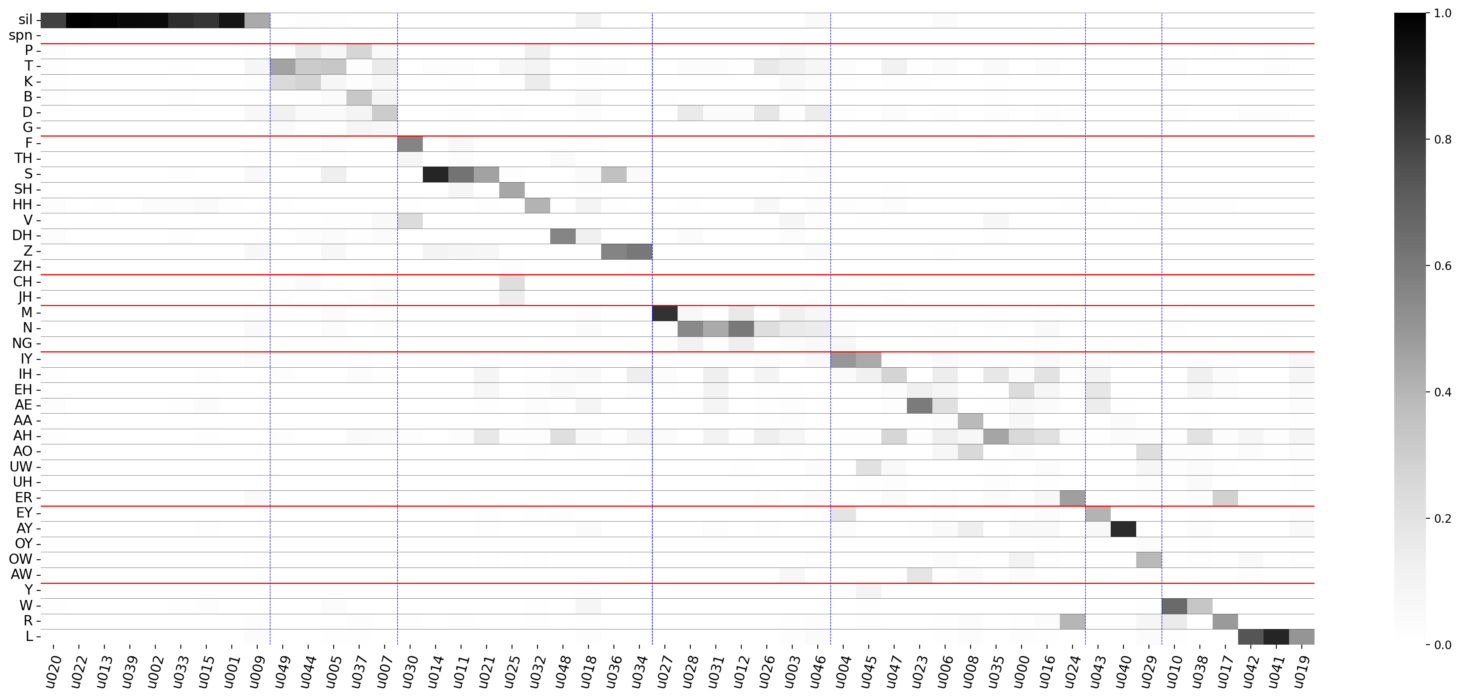
\includegraphics[width=0.8\linewidth]{figures/ch4figs/hub-u050-ap0000-givenunit-byphn.png}
                    \caption{離散單元}
                    \label{subfig:hub-u050-ap0000-givenunit-byphn}
                \end{subfigure}
                \vfill
                \begin{subfigure}{\textwidth}
                    \centering
                    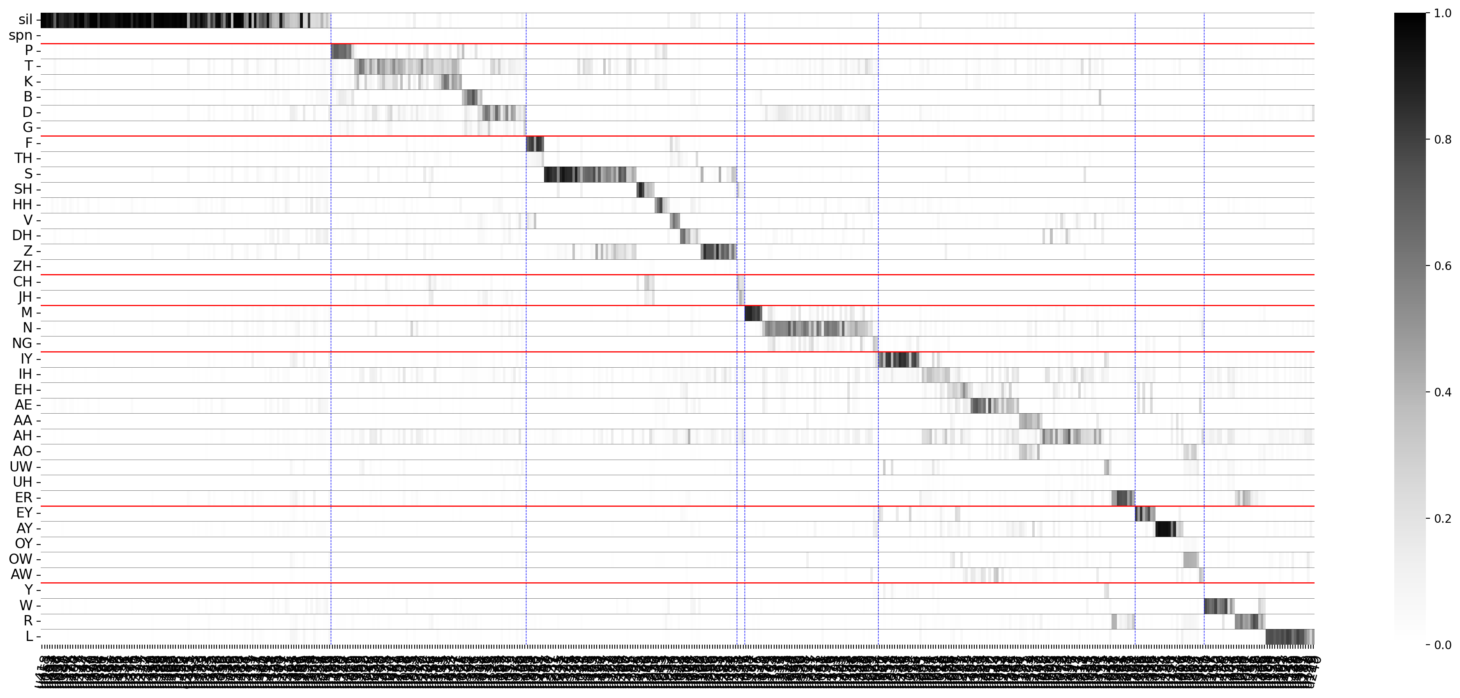
\includegraphics[width=0.8\linewidth]{figures/ch4figs/hub-u050-ap0500-givenunit-byphn.png}
                    \caption{500 種\textcolor{red}{次詞單位}}
                    \label{subfig:hub-u050-ap0500-givenunit-byphn}
                \end{subfigure}
                \vfill
                \begin{subfigure}{\textwidth}
                    \centering
                    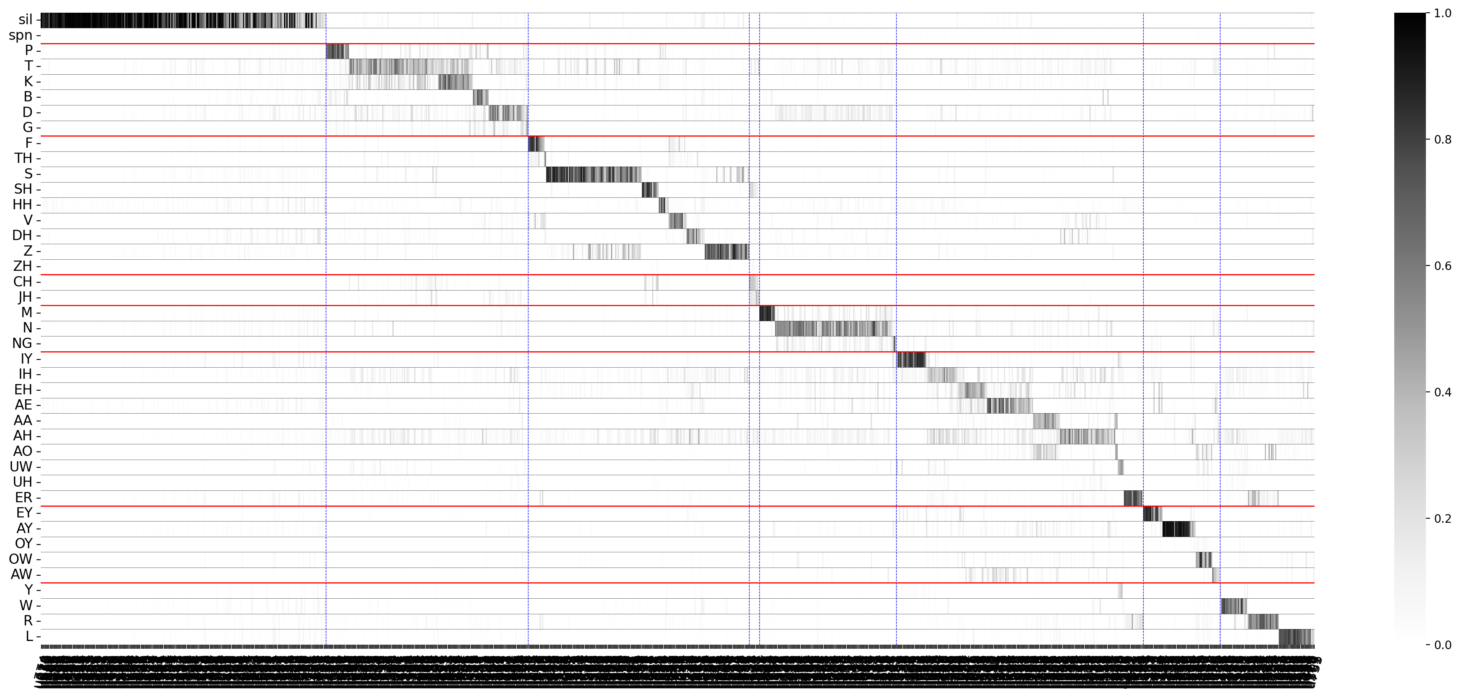
\includegraphics[width=0.8\linewidth]{figures/ch4figs/hub-u050-ap1000-givenunit-byphn.png}
                    \caption{1000 種\textcolor{red}{次詞單位}}
                    \label{subfig:hub-u050-ap1000-givenunit-byphn}
                \end{subfigure}

                \caption{HuBERT 表徵在 K-平均演算法使用分群數 50 後,}
                比較不同\textcolor{red}{次詞單位}數量的條件機率分佈 $p_{y|z}(i | j)$ 熱圖
                \label{fig:hub-u050-comparisons}
            \end{figure}
        }
        {
            \begin{figure}
                \centering
                \begin{subfigure}{\textwidth}
                    \centering
                    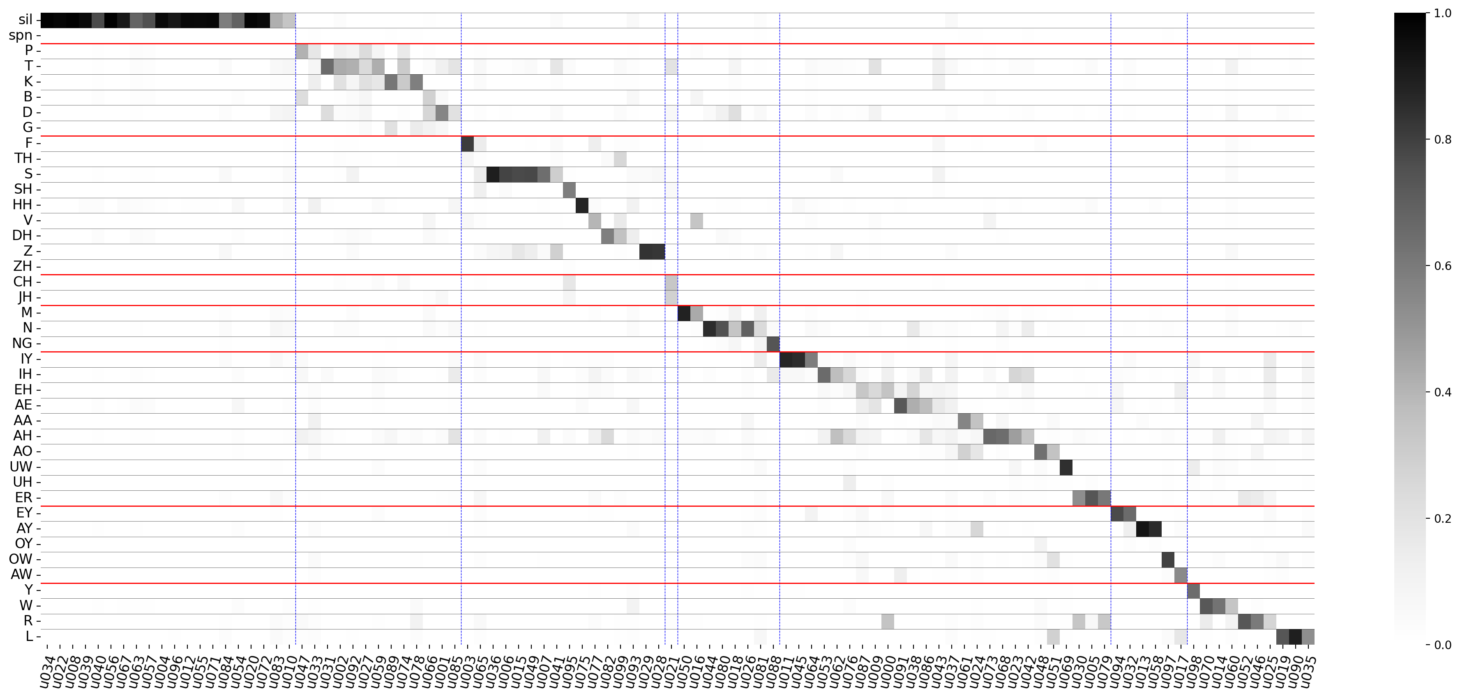
\includegraphics[width=0.8\linewidth]{figures/ch4figs/hub-u100-ap0000-givenunit-byphn.png}
                    \caption{離散單元}
                    \label{subfig:hub-u100-ap0000-givenunit-byphn}
                \end{subfigure}
                \vfill
                \begin{subfigure}{\textwidth}
                    \centering
                    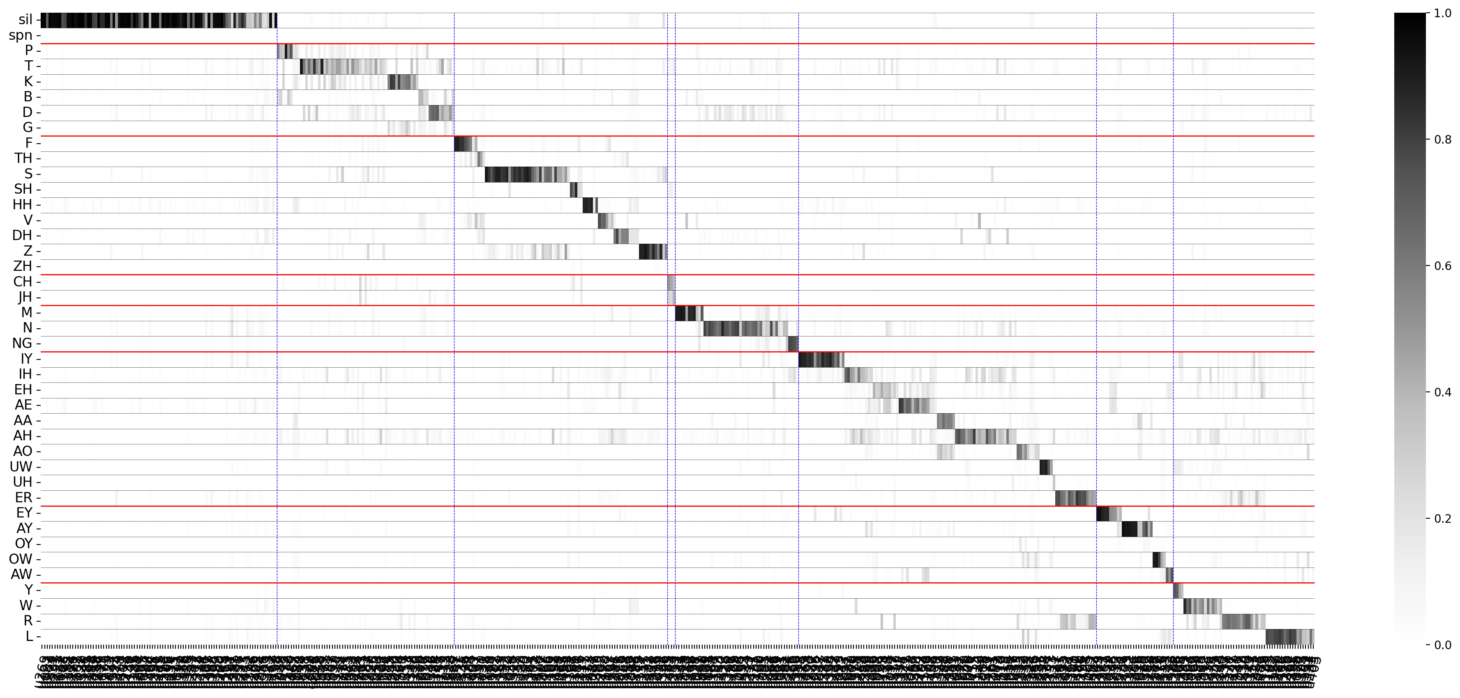
\includegraphics[width=0.8\linewidth]{figures/ch4figs/hub-u100-ap0500-givenunit-byphn.png}
                    \caption{500 種\textcolor{red}{次詞單位}}
                    \label{subfig:hub-u100-ap0500-givenunit-byphn}
                \end{subfigure}
                \vfill
                \begin{subfigure}{\textwidth}
                    \centering
                    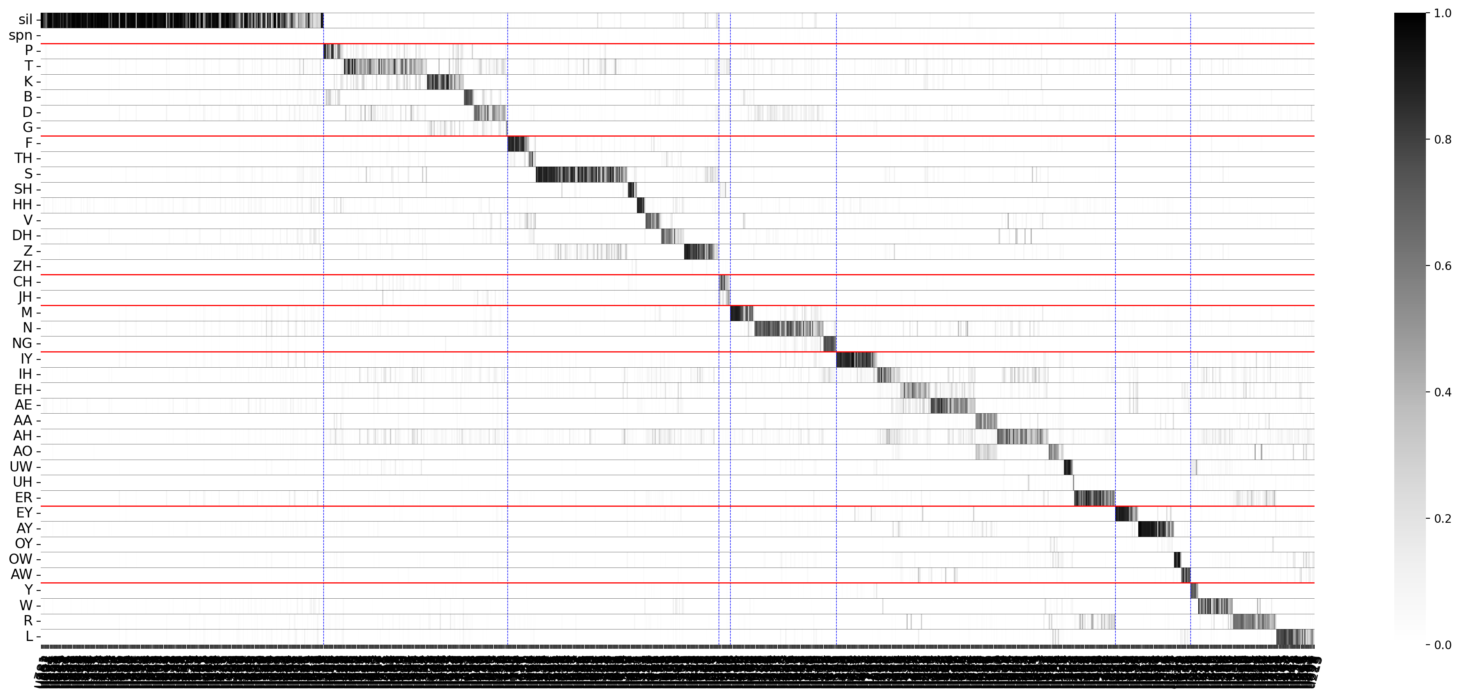
\includegraphics[width=0.8\linewidth]{figures/ch4figs/hub-u100-ap1000-givenunit-byphn.png}
                    \caption{1000 種\textcolor{red}{次詞單位}}
                    \label{subfig:hub-u100-ap1000-givenunit-byphn}
                \end{subfigure}

                \caption{HuBERT 表徵在 K-平均演算法使用分群數 100 後,}
                比較不同\textcolor{red}{次詞單位}數量的條件機率分佈 $p_{y|z}(i | j)$ 熱圖
                \label{fig:hub-u100-comparisons}
            \end{figure}
        }
    }
    {
        \begin{figure}
            \centering
            \begin{subfigure}{\textwidth}
                \centering
                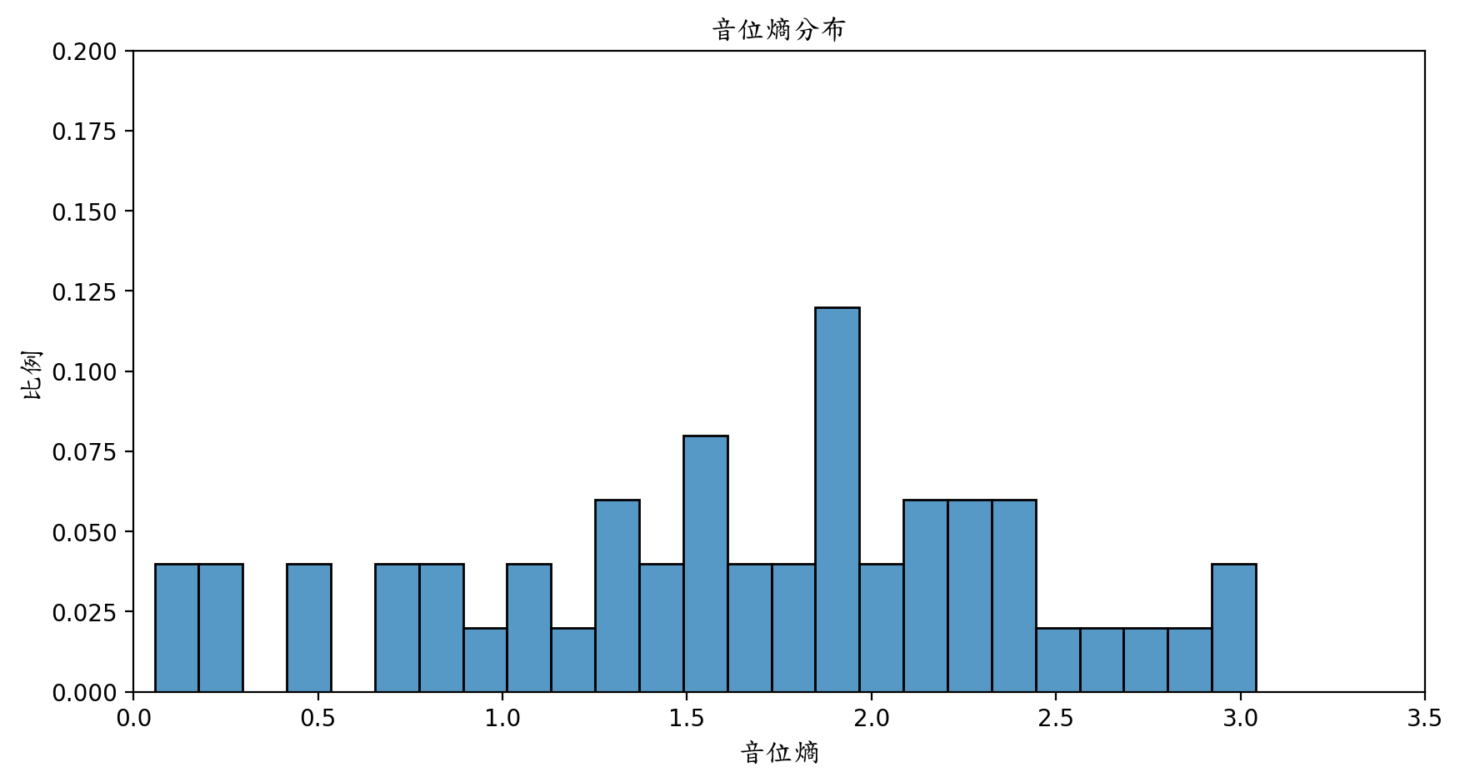
\includegraphics[width=0.7\linewidth]{figures/ch4figs/hub-u050-ap0000-phnent-hist.png}
                \caption{離散單元}
                \label{subfig:hub-u050-ap0000-phnent-hist}
            \end{subfigure}
            \vfill
            \begin{subfigure}{\textwidth}
                \centering
                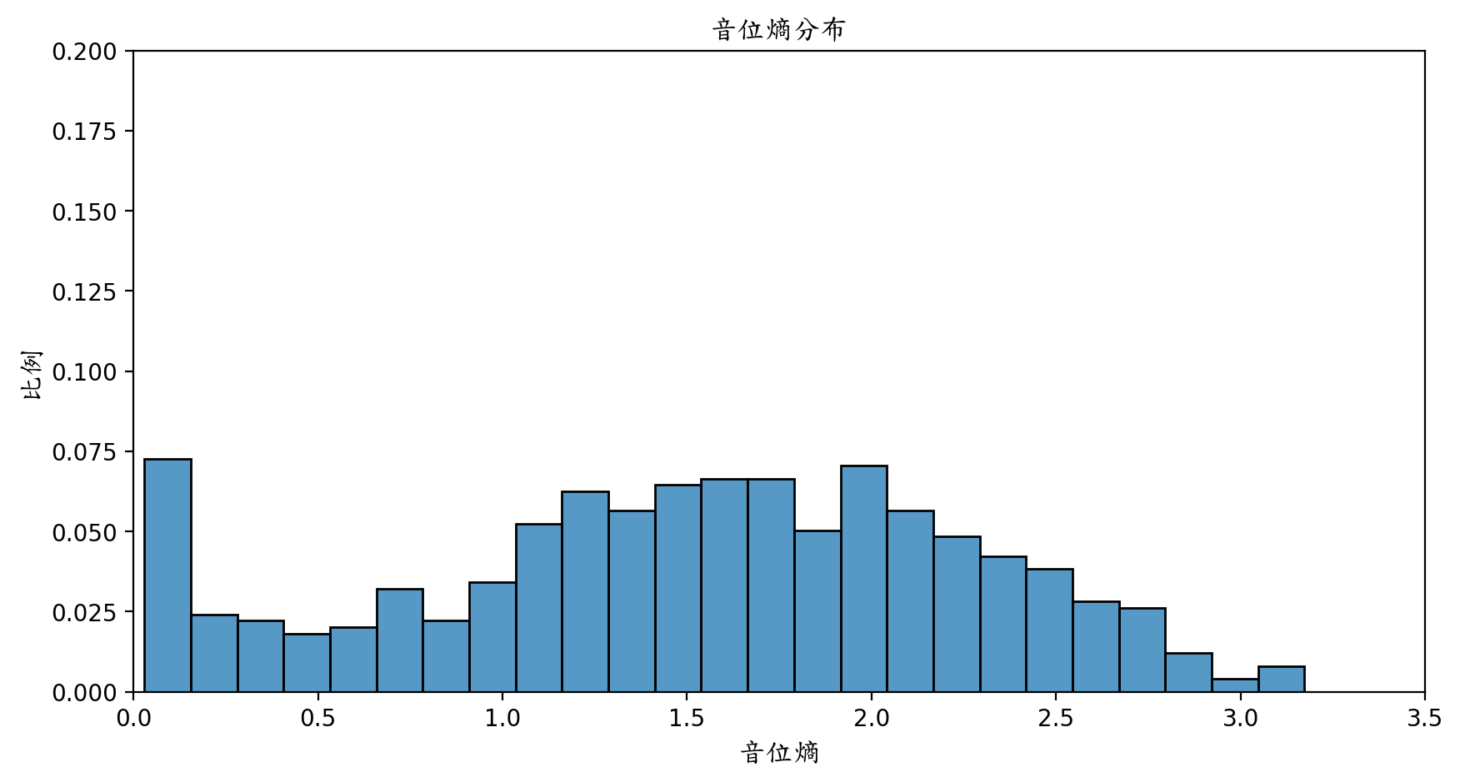
\includegraphics[width=0.7\linewidth]{figures/ch4figs/hub-u050-ap0500-phnent-hist.png}
                \caption{500 種\textcolor{red}{次詞單位}}
                \label{subfig:hub-u050-ap0500-phnent-hist}
            \end{subfigure}
            \vfill
            \begin{subfigure}{\textwidth}
                \centering
                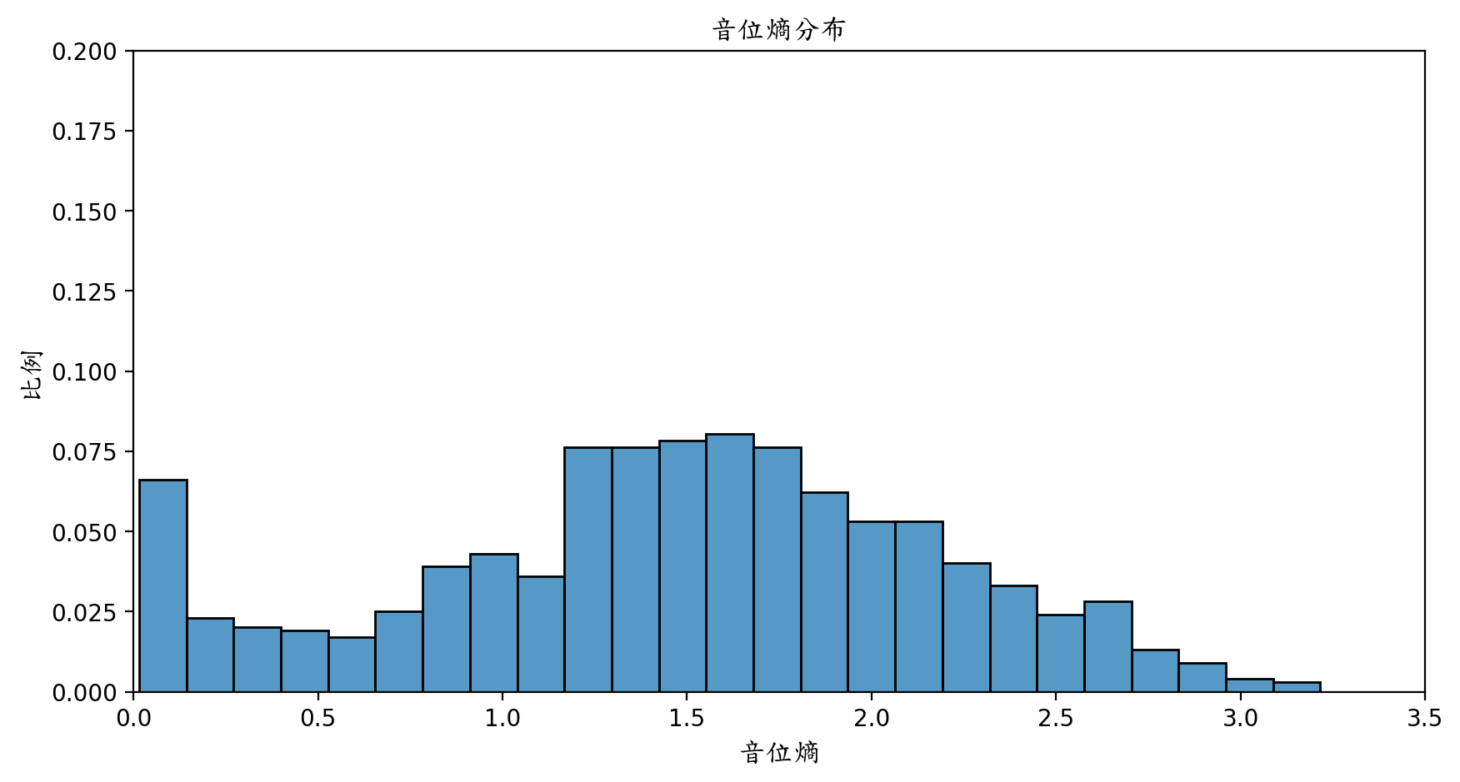
\includegraphics[width=0.7\linewidth]{figures/ch4figs/hub-u050-ap1000-phnent-hist.png}
                \caption{1000 種\textcolor{red}{次詞單位}}
                \label{subfig:hub-u050-ap1000-phnent-hist}
            \end{subfigure}

            \caption{HuBERT 表徵在 K-平均演算法使用分群數 50 後,}
            比較不同\textcolor{red}{次詞單位}數量的音位條件熵 $H(y|z)$ 直方圖
            \label{fig:hub-u050-hist-comparisons}
        \end{figure}

        \begin{figure}
            \centering
            \begin{subfigure}{\textwidth}
                \centering
                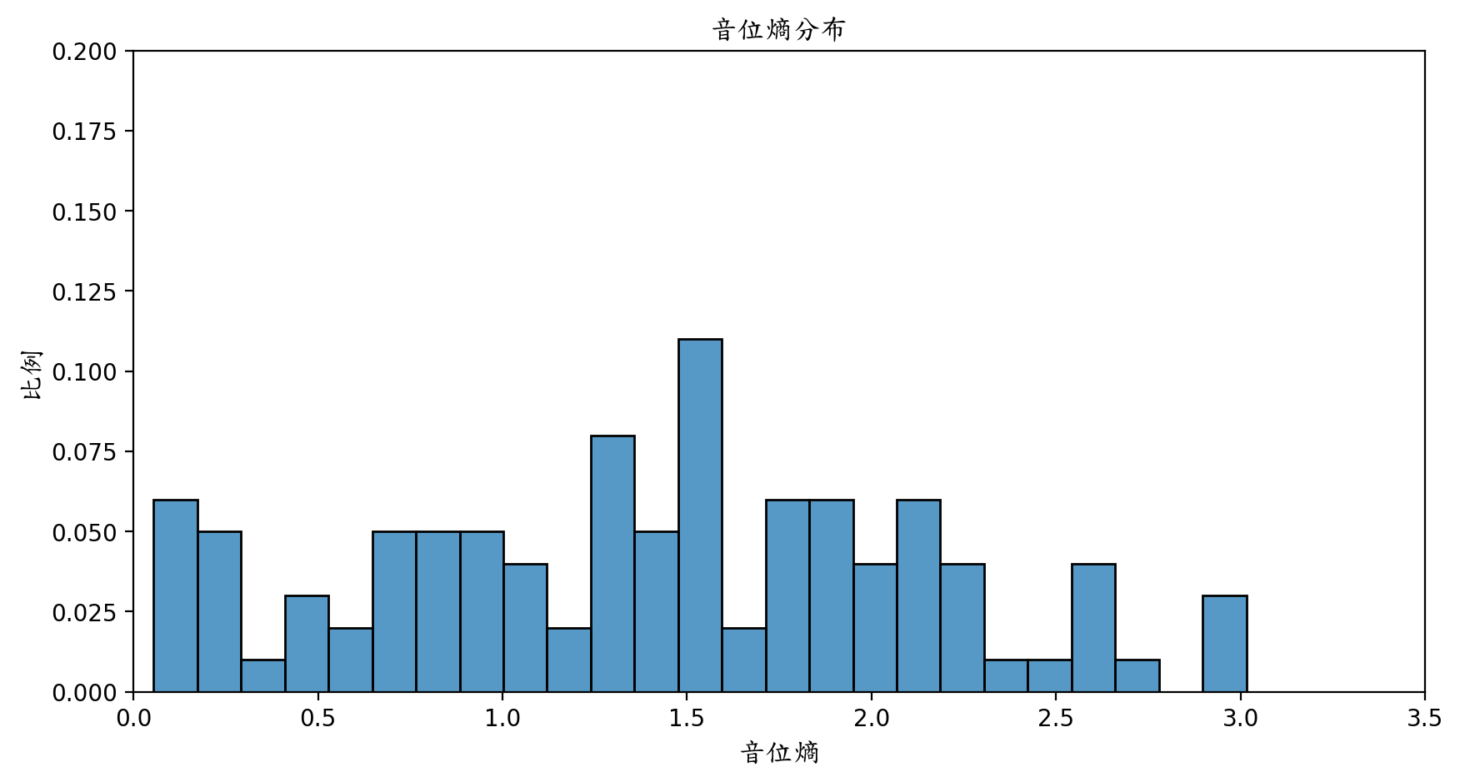
\includegraphics[width=0.7\linewidth]{figures/ch4figs/hub-u100-ap0000-phnent-hist.png}
                \caption{離散單元}
                \label{subfig:hub-u100-ap0000-phnent-hist}
            \end{subfigure}
            \vfill
            \begin{subfigure}{\textwidth}
                \centering
                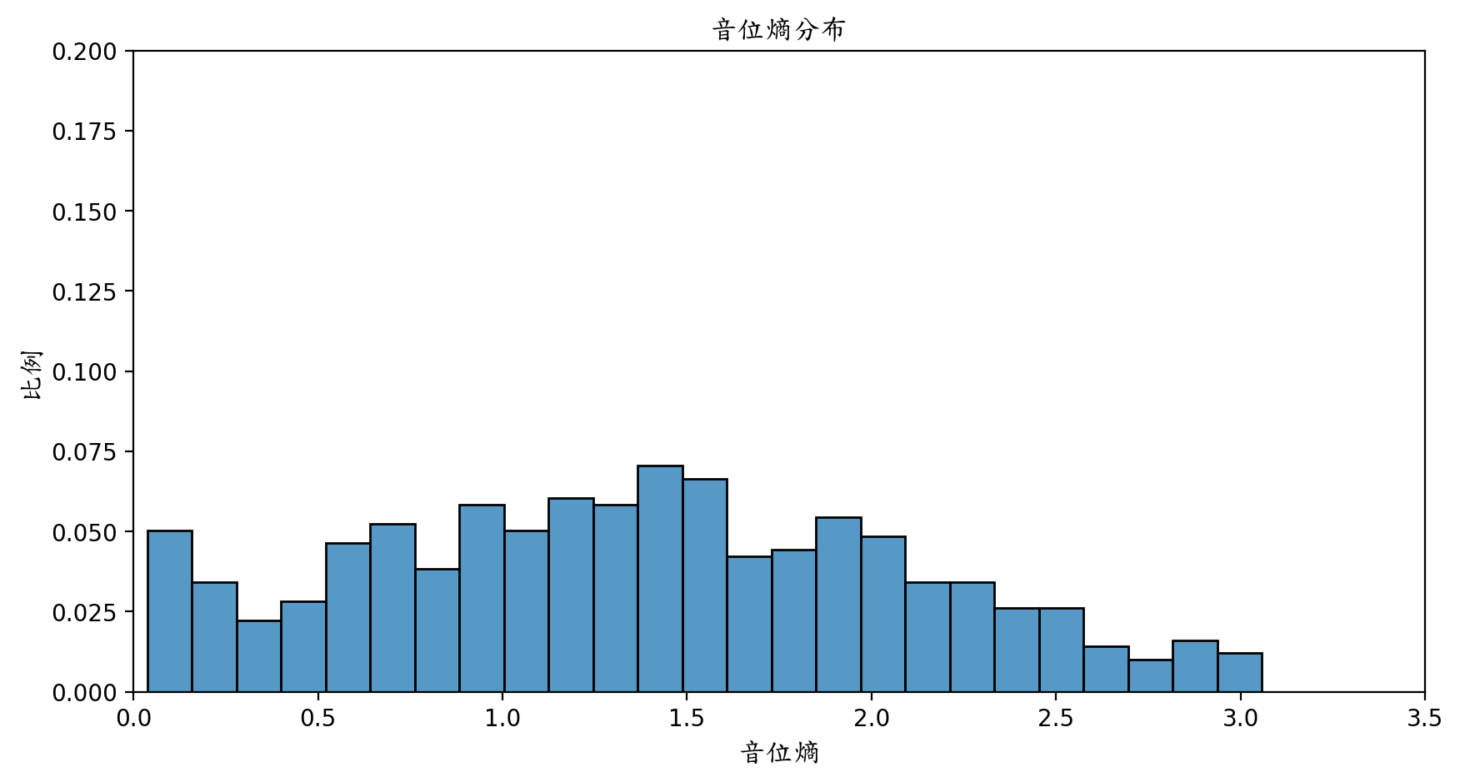
\includegraphics[width=0.7\linewidth]{figures/ch4figs/hub-u100-ap0500-phnent-hist.png}
                \caption{500 種\textcolor{red}{次詞單位}}
                \label{subfig:hub-u100-ap0500-phnent-hist}
            \end{subfigure}
            \vfill
            \begin{subfigure}{\textwidth}
                \centering
                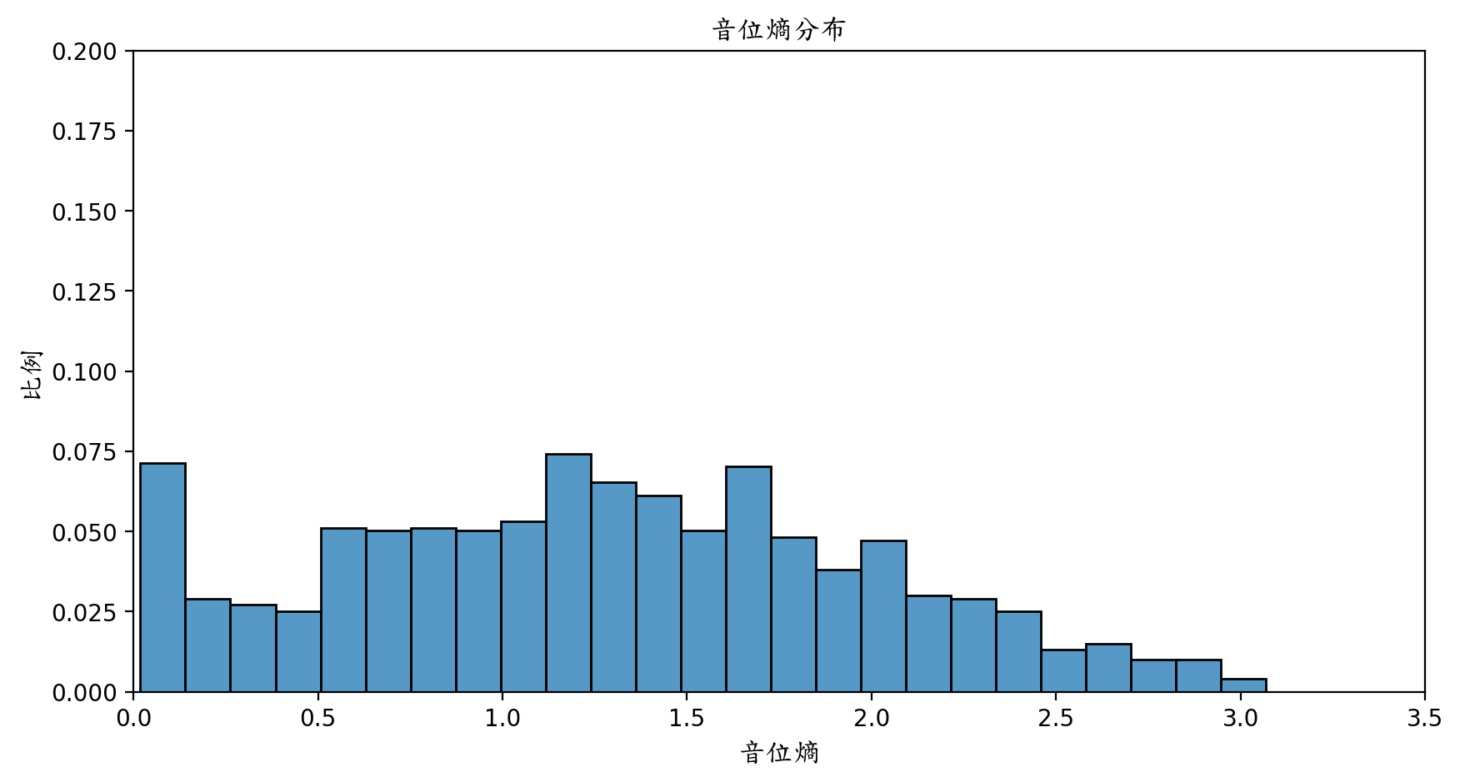
\includegraphics[width=0.7\linewidth]{figures/ch4figs/hub-u100-ap1000-phnent-hist.png}
                \caption{1000 種\textcolor{red}{次詞單位}}
                \label{subfig:hub-u100-ap1000-phnent-hist}
            \end{subfigure}

            \caption{HuBERT 表徵在 K-平均演算法使用分群數 100 後,}
            比較不同\textcolor{red}{次詞單位}數量的音位條件熵 $H(y|z)$ 直方圖
            \label{fig:hub-u100-hist-comparisons}
        \end{figure}
    }

    {
        \begin{figure}
             \centering
             \begin{subfigure}{\textwidth}
                 \centering
                 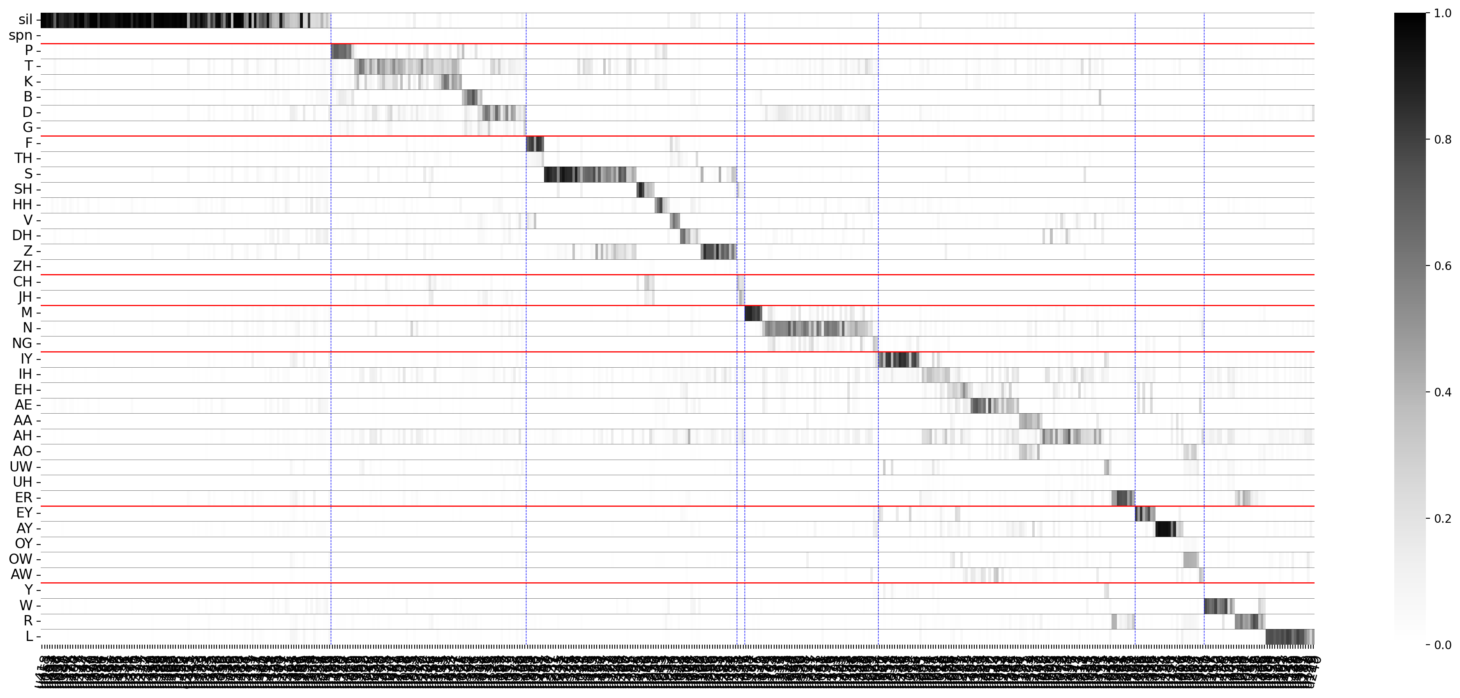
\includegraphics[width=1\linewidth]{figures/ch4figs/hub-u050-ap0500-givenunit-byphn.png}
                 \caption{分群數 50}
                 \label{subfig:hub-u050-ap0500-givenunit-byphn--picked}
             \end{subfigure}
             \vfill
             \begin{subfigure}{\textwidth}
                 \centering
                 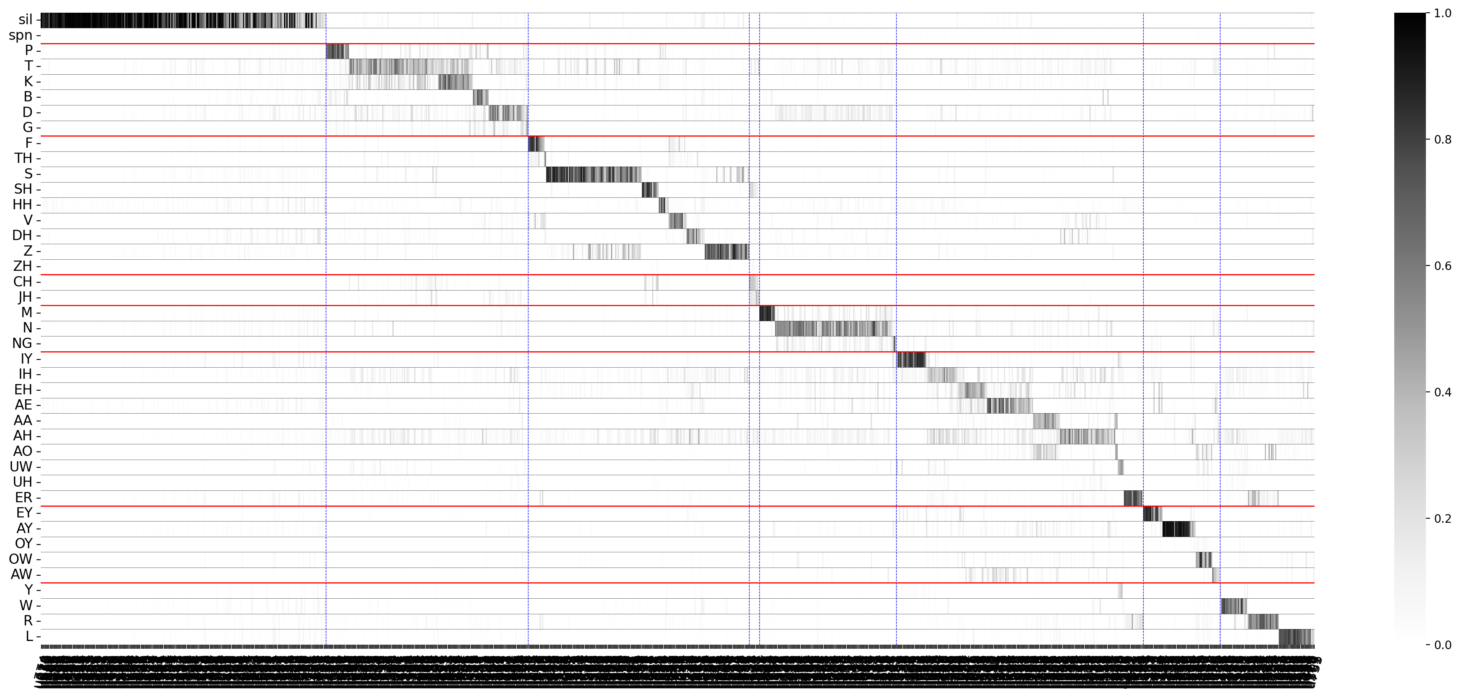
\includegraphics[width=1\linewidth]{figures/ch4figs/hub-u050-ap1000-givenunit-byphn.png}
                 \caption{分群數 100}
                 \label{subfig:hub-u100-ap0500-givenunit-byphn--picked}
             \end{subfigure}
             \caption{比較同樣 500 種\textcolor{red}{次詞單位}的\textcolor{red}{聲學片段}模型,著重比較 HuBERT 表徵}
             在 K-平均演算法使用分群數 50 與 100 的條件機率熱圖 $p_{y|z}(i|j)$ 差異
             \label{fig:check-ap0500}
        \end{figure}
    }

    {
        \begin{table}
            \centering
            \begin{subtable}{\textwidth}
                \centering
                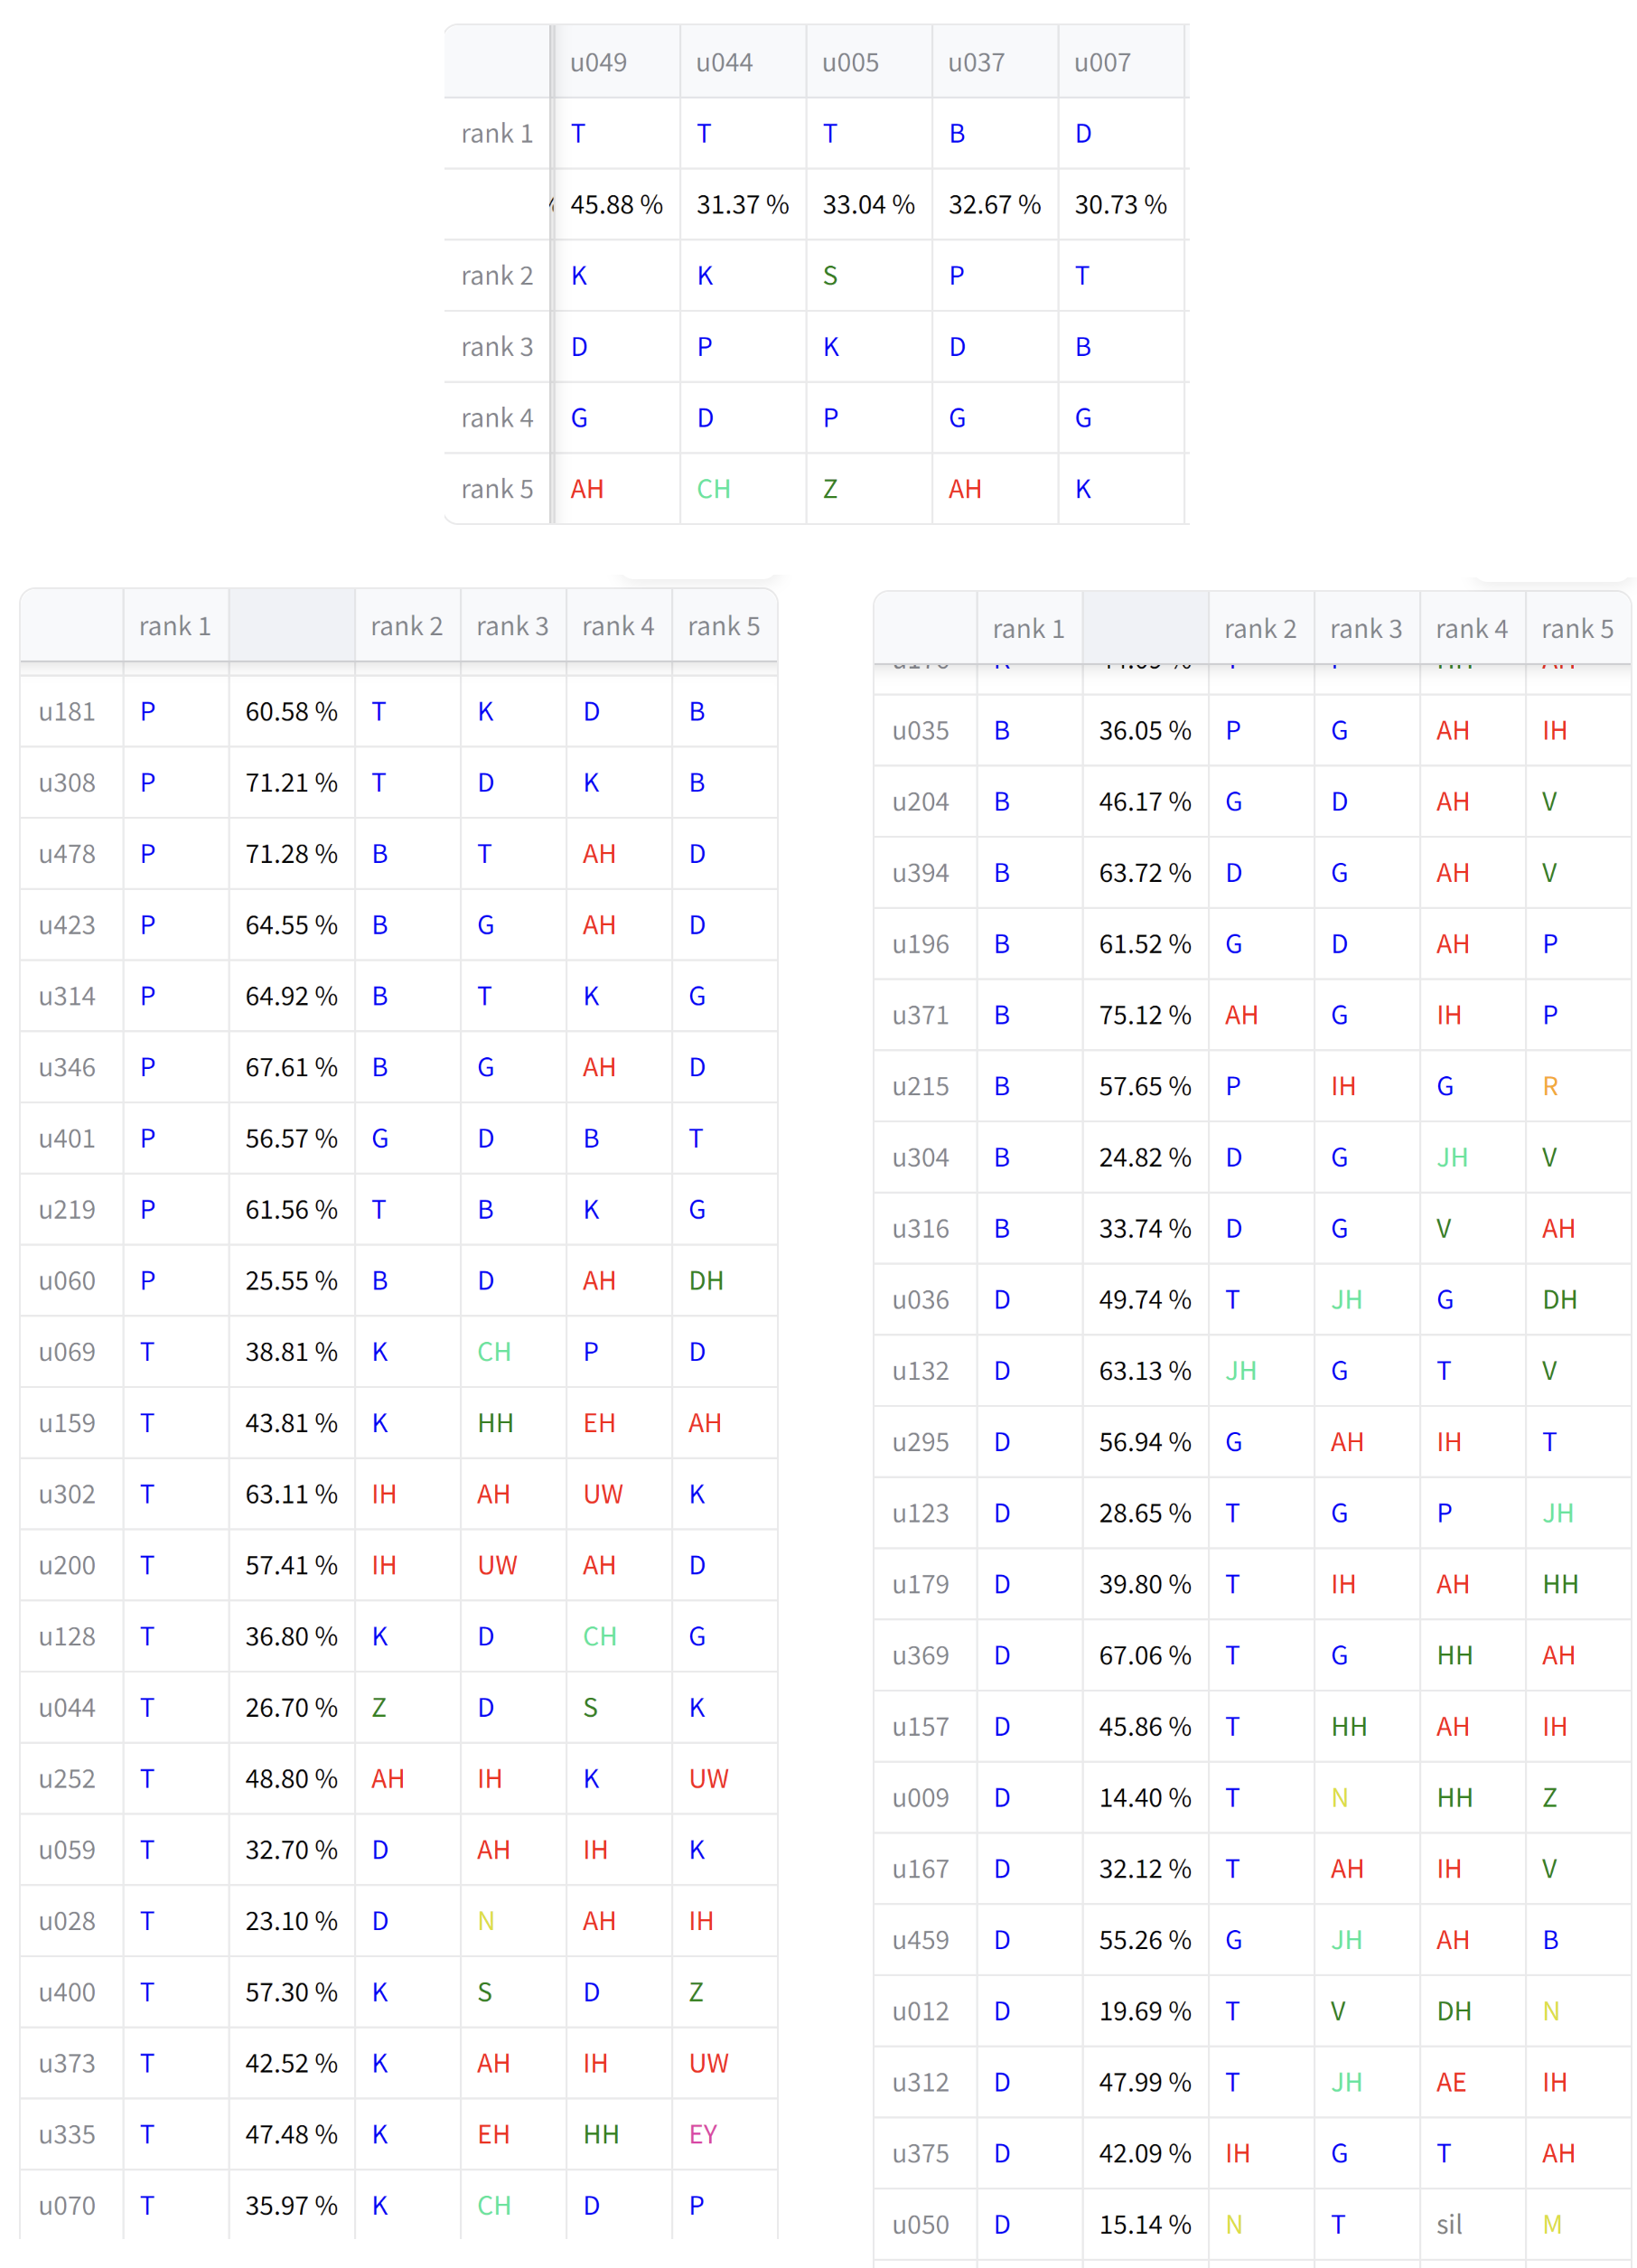
\includegraphics[width=0.8\linewidth]{figures/ch4figs/plo_phn.png}
                \caption{塞音}
                \label{subtabfig:hub-u050-ap0500-ploobs}
            \end{subtable}

            \caption{HuBERT 表徵、K-平均演算法分群數 50,比較單一離散單元與}
            使用 500 種\textcolor{red}{次詞單位},依據不同音位分類比較\textcolor{red}{符記}各自對應的前五高音位 \\
            上半部為離散單元,下半部為\textcolor{red}{聲學片段}。 \\
            圖中的百分比為最高機率音位的條件機率 $p_{y|z}(i^*(j)|j)$
            \label{tabfig:hub-u050-phnobserver}
        \end{table}

        \begin{table}
            \ContinuedFloat
            \centering
            \begin{subtable}{\textwidth}
                \centering
                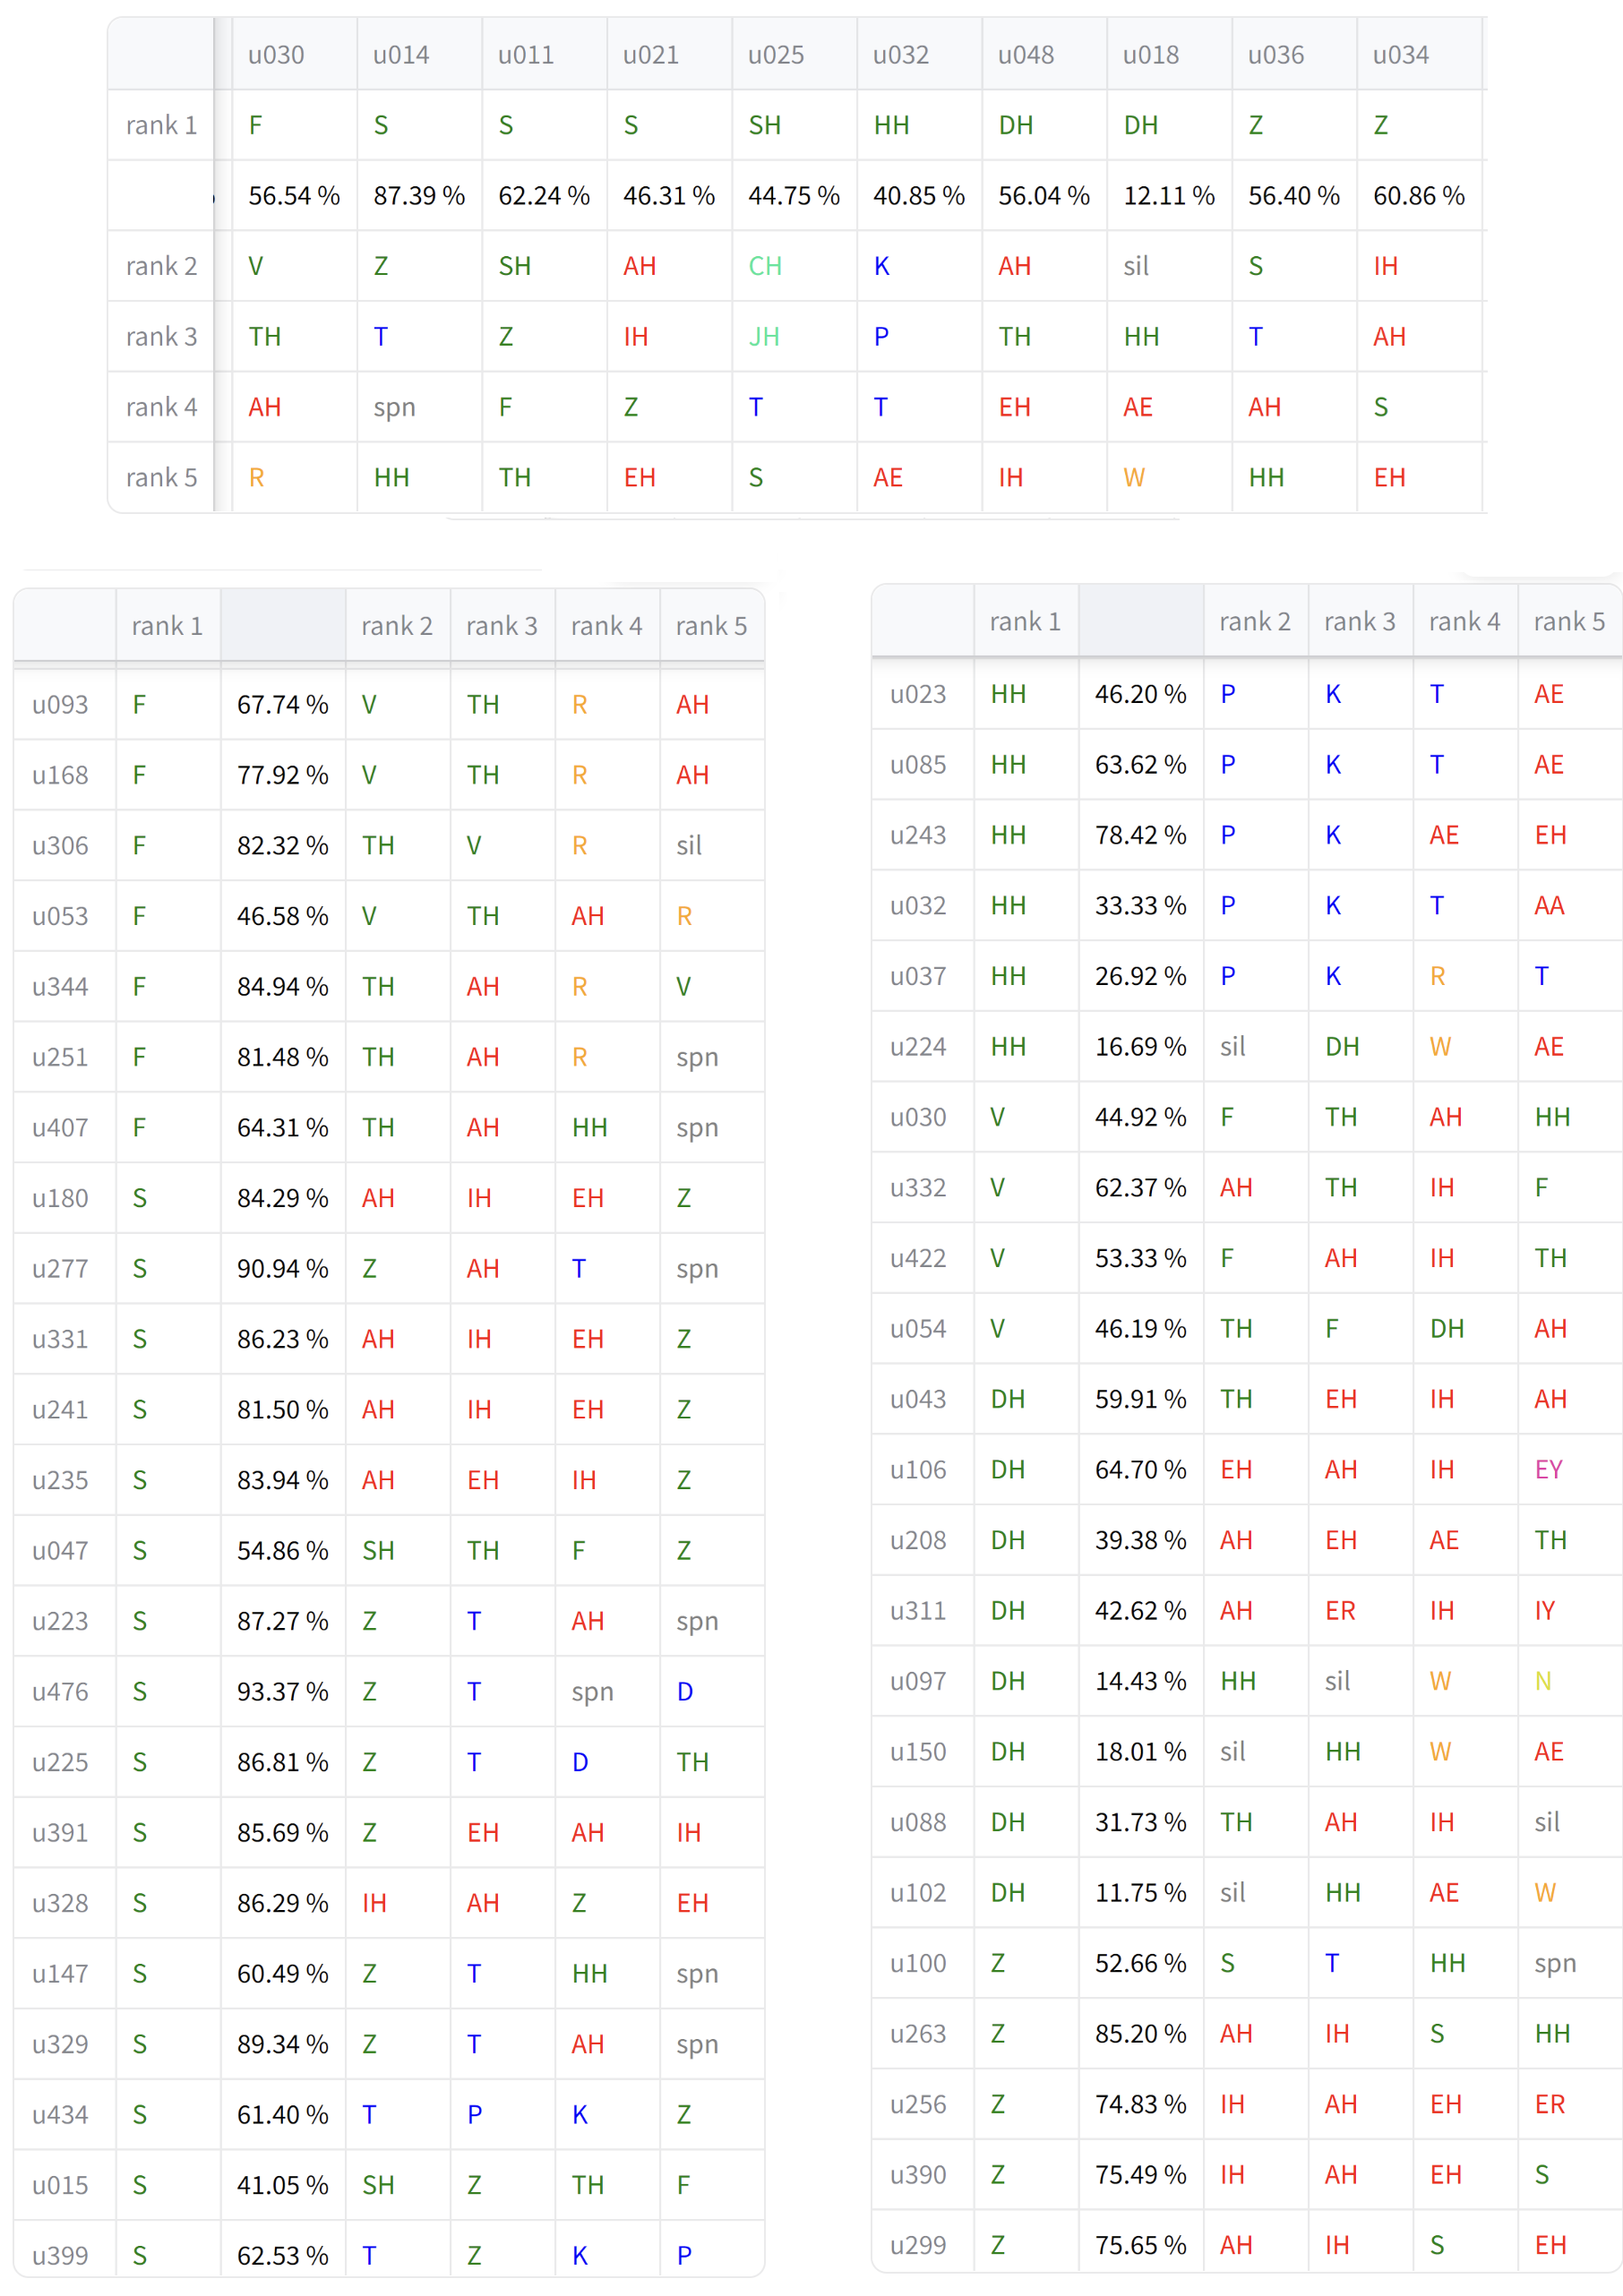
\includegraphics[width=0.8\linewidth]{figures/ch4figs/fri_phn.png}
                \caption{擦音}
                \label{subtabfig:hub-u050-ap0500-friobs}
            \end{subtable}

            \label{tabfig:hub-u050-phnobserver--2}
        \end{table}

        \begin{table}
            \ContinuedFloat
            \centering
            \begin{subtable}{\textwidth}
                \centering
                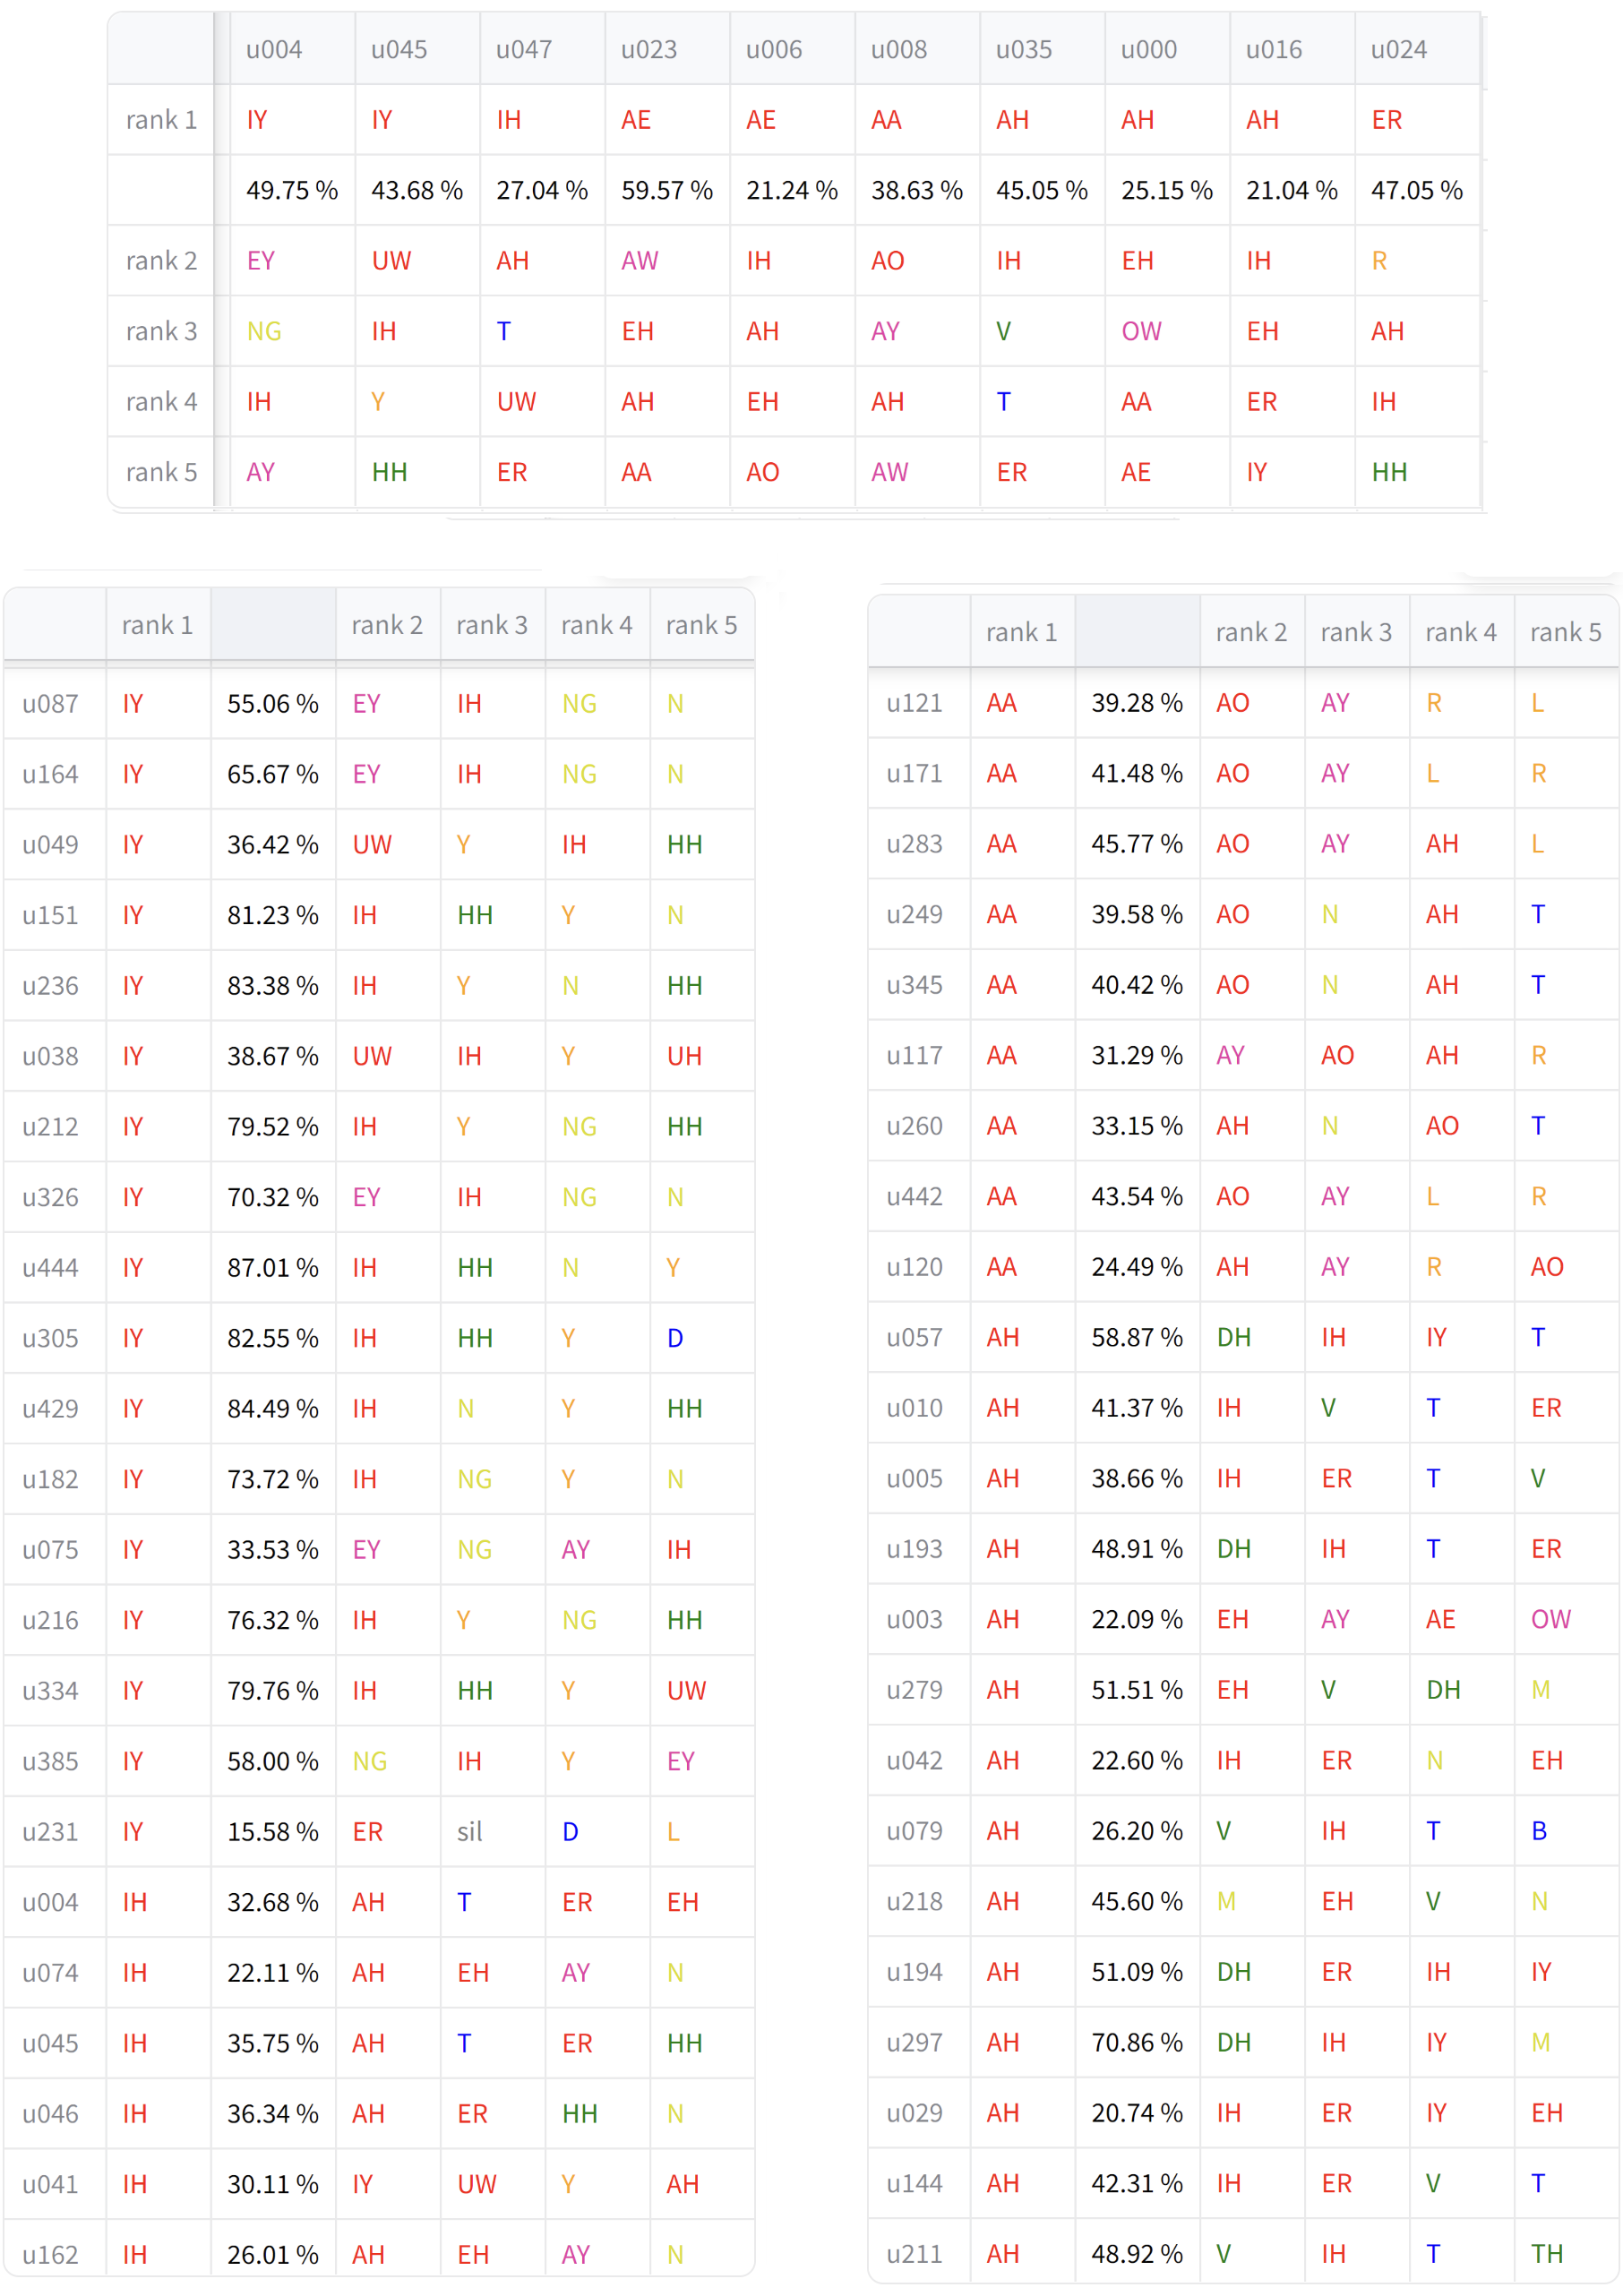
\includegraphics[width=0.8\linewidth]{figures/ch4figs/vow_phn.png}
                \caption{單元音}
                \label{subtabfig:hub-u050-ap0500-vowobs}
            \end{subtable}

            \label{tabfig:hub-u050-phnobserver--3}
        \end{table}
    }

    {
        \begin{table}
            \centering
            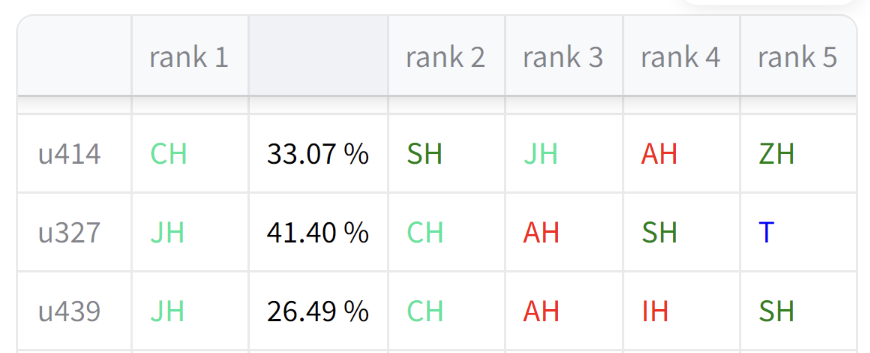
\includegraphics[width=0.8\linewidth]{figures/ch4figs/aff-hub50-500.png}
            \caption{對 HuBERT 分群數 50 離散單元取得 500 種\textcolor{red}{次詞單位}後,}
            對應到塞擦音的\textcolor{red}{聲學片段}之音位條件機率排名
            \label{tabfig:aff}
        \end{table}

        \begin{table}[!htbp]
            \centering

            \begin{subtable}[t]{\textwidth}
                \centering
                \begin{tabular}{|c|c|c|} \hline
                    \textcolor{red}{符記}種數  & 音位分類純度    & 以音位分類標註之分群純度    \\ \hline
                                     離散單元  &         0.7006  &            \textbf{0.1509}  \\ \hline
                                         500   &         0.7116  &                    0.0340   \\ \hline
                                        1000   & \textbf{0.7186} &                    0.0226   \\ \hline
                                        8000   &         0.7080  &                    0.0119   \\ \hline
                                       10000   &         0.7048  &                    0.0113   \\ \hline
                                       20000   &         0.6929  &                    0.0089   \\ \hline
                \end{tabular}
                \caption{群數 = 50}
                \label{subtab:ch4-new-hubert-pcls-clu050}
            \end{subtable}

            \vfill

            \begin{subtable}[t]{\textwidth}
                \centering
                \begin{tabular}{|c|c|c|} \hline
                    \textcolor{red}{符記}種數  & 音位分類純度    & 以音位分類標註之分群純度 \\ \hline
                                     離散單元  & \textbf{0.7584} & \textbf{0.0882}          \\ \hline
                                          500  &        0.7578   &         0.0326           \\ \hline
                                         1000  &        0.7576   &         0.0223           \\ \hline
                                         8000  &        0.7382   &         0.0097           \\ \hline
                                        10000  &        0.7346   &         0.0090           \\ \hline
                                        20000  &        0.7235   &         0.0074           \\ \hline
                \end{tabular}
                \caption{群數 = 100}
                \label{subtab:ch4-new-hubert-pcls-clu100}
            \end{subtable}

            \caption{HuBERT 模型在不同詞表大小時的語音學類別分析數據}
            \label{tab:new--hubert-pcls-results}
        \end{table}
    }


    {
        \begin{table}
            \centering
            \begin{subtable}{\textwidth}
                \centering
                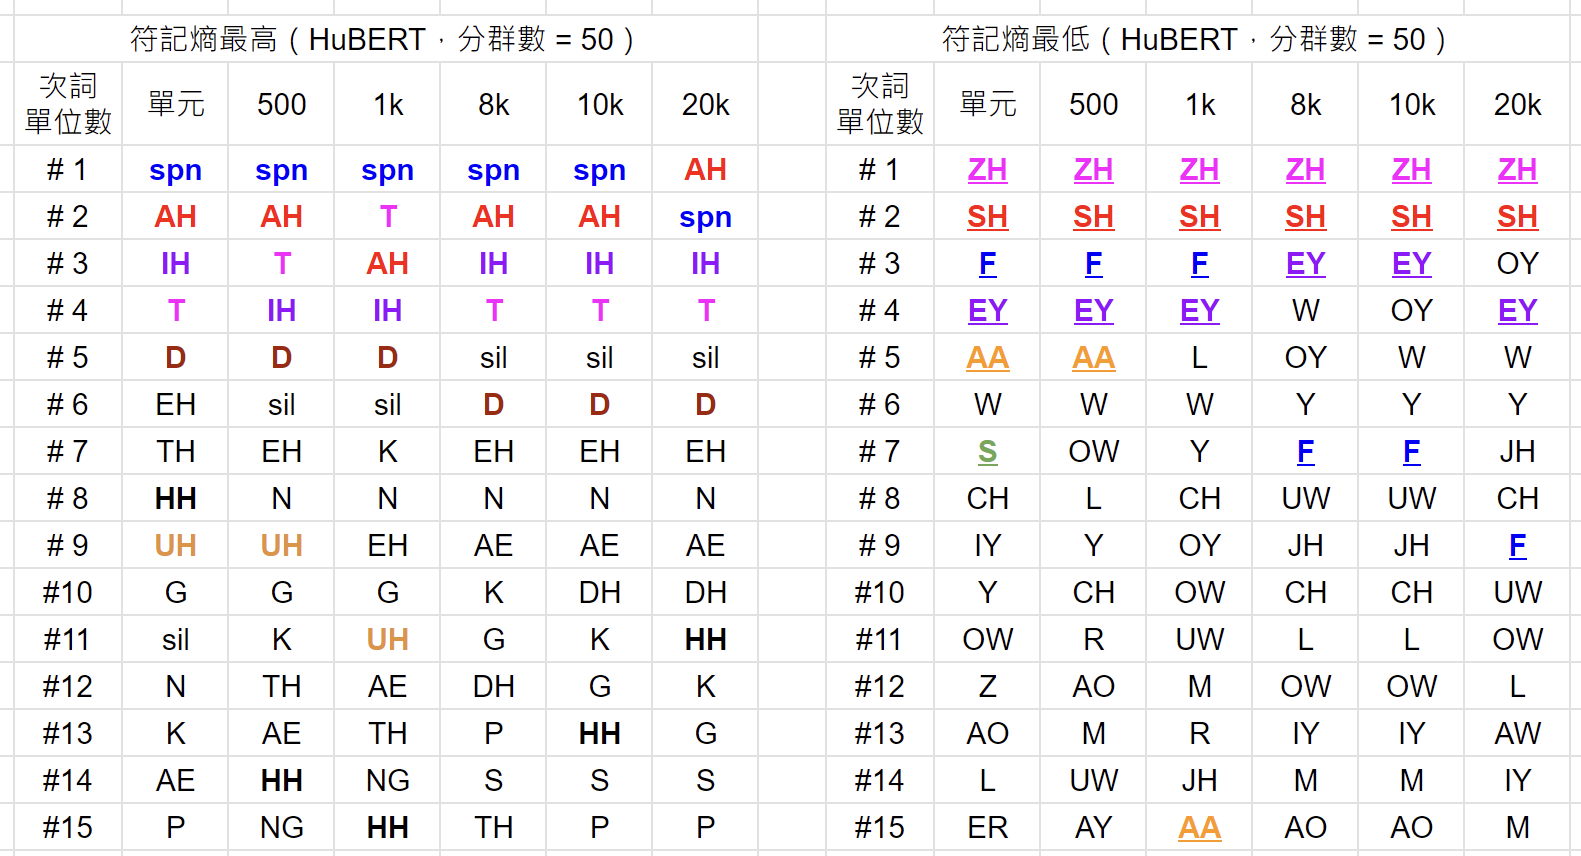
\includegraphics[width=1\linewidth]{figures/ch4figs/phnrank-hub50pcs.png}
                \caption{分群數 = 50}
                \label{subtabfig:hub-u050-phnrank-hub50pcs}
            \end{subtable}
            \vfill
            \begin{subtable}{\textwidth}
                \centering
                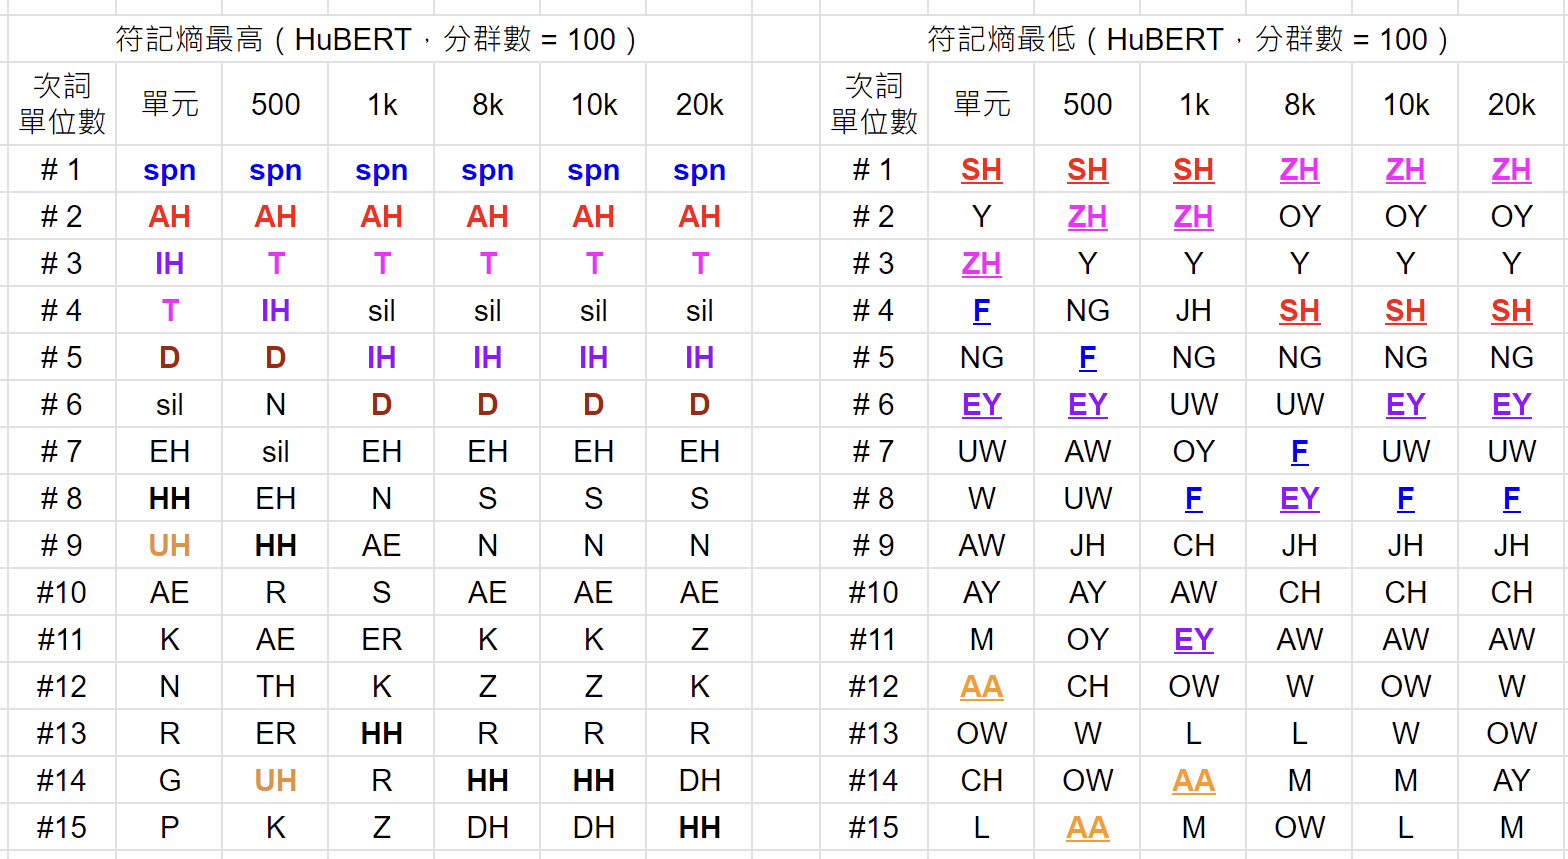
\includegraphics[width=1\linewidth]{figures/ch4figs/phnrank-hub100pcs.png}
                \caption{分群數 = 100}
                \label{subtabfig:hub-u050-phnrank-hub100pcs}
            \end{subtable}
    
            \caption{HuBERT 表徵、K-平均演算法分群數 50 和 100,}
            比較不同\textcolor{red}{次詞單位}種數時,\textcolor{red}{符記}熵最高與最低的音位排名
            \label{tabfig:hub-u050-phnrank}
        \end{table}
    }

    {
        \begin{table}
            \centering
            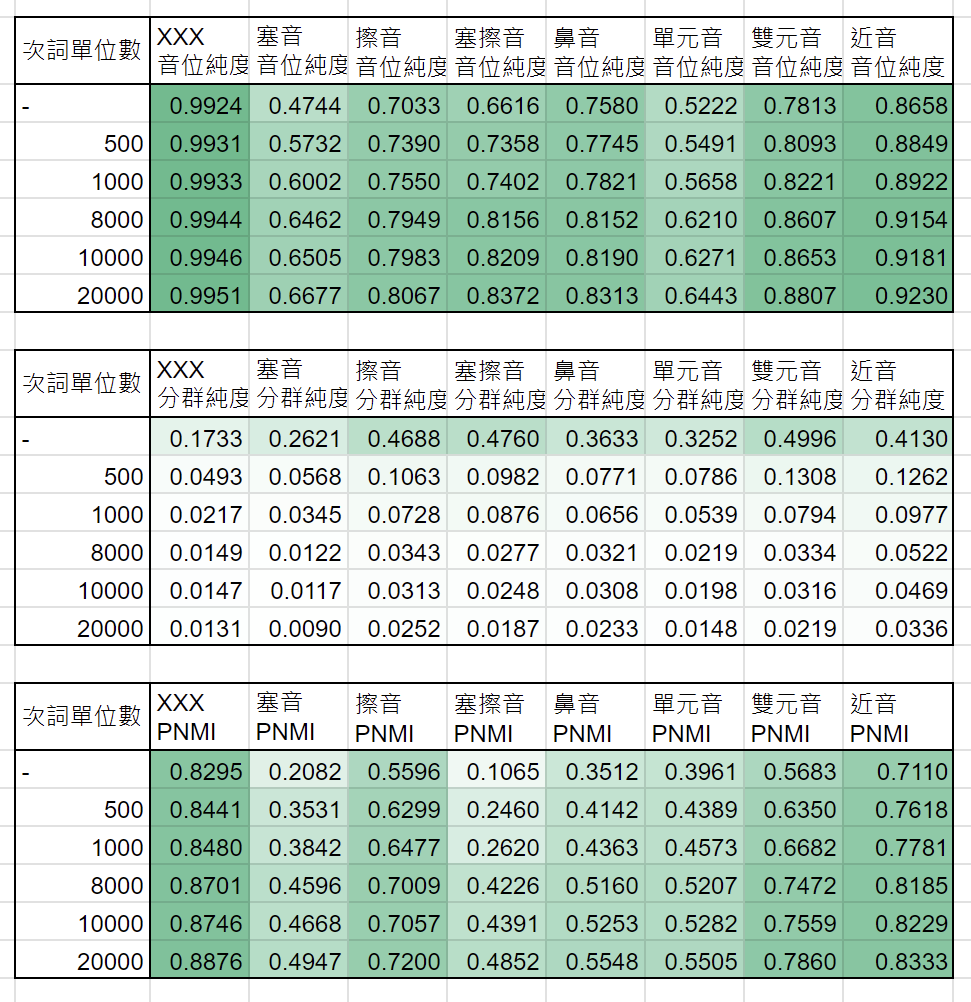
\includegraphics[width=1\linewidth]{figures/ch4figs/hub50-ap-detailedpur.png}
            \caption{HuBERT 分群數 50 的離散單元,以不同\textcolor{red}{符記}種數取得\textcolor{red}{聲學片段}後,}
            按照音位分類分開各自計算的純度與相互資訊
            \label{tabfig:hub50-ap-detailedpur}
        \end{table}

        \begin{table}
            \centering
            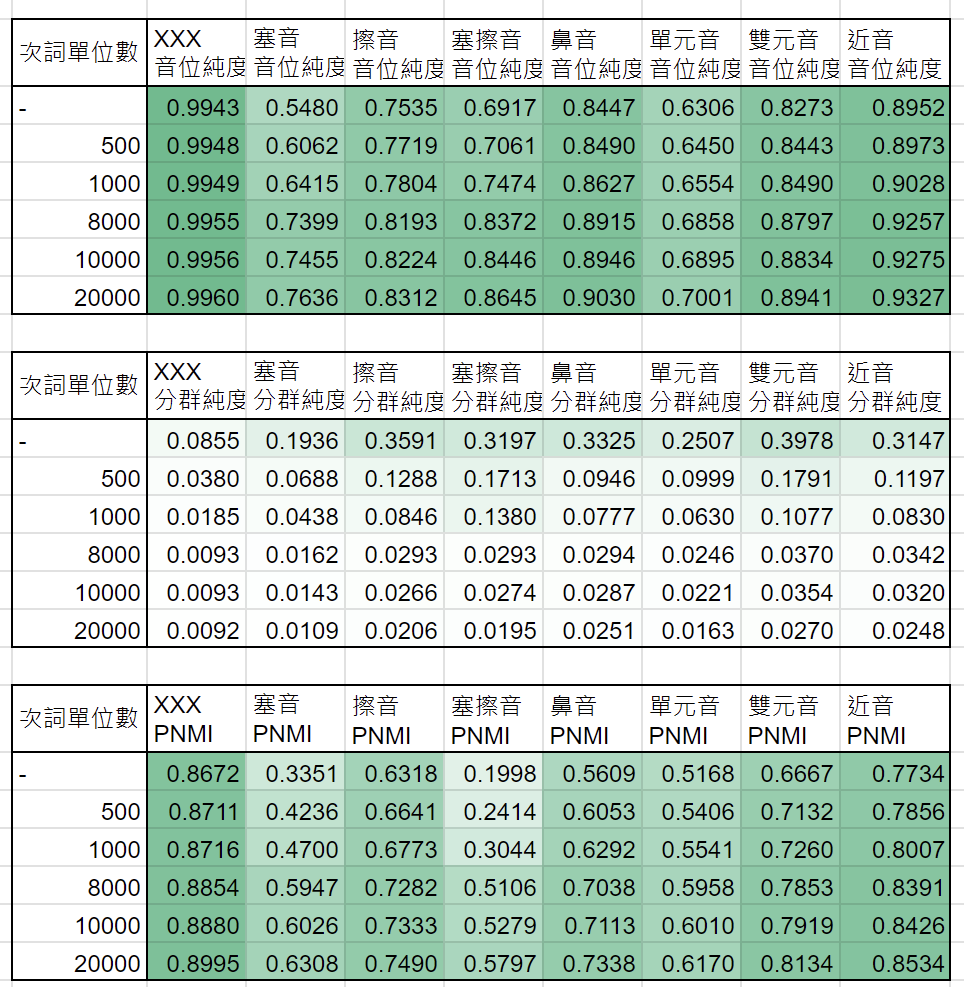
\includegraphics[width=1\linewidth]{figures/ch4figs/hub100-ap-detailedpur.png}
            \caption{HuBERT 分群數 100 的離散單元,以不同\textcolor{red}{符記}種數取得\textcolor{red}{聲學片段}後,}
            按照音位分類分開各自計算的純度與相互資訊
            \label{tabfig:hub100-ap-detailedpur}
        \end{table}
    }


\section{分析結果} 

  承繼上一個章節的分析方法,我們先將純度等數據與條件機率熱圖 $p_{y|z}(i | j)$ \footnote{由於共同機率分佈熱圖 $p_{yz}$ 的數值對於觀察\textcolor{red}{符記}對應到音位的關係較不明顯,因此仿照 SpeechTokenizer \cite{zhang2024speechtokenizer}、DinoSR \cite{liu2024dinosr} 等論文使用 $p_{y|z}(i | j)$ 呈現。} 兩者互相對照,並以語音學排序呈現,觀察\textcolor{red}{聲學片段}與音位之間兩者的分佈關係。

\subsection{由\textcolor{red}{聲學片段}角度探討}

\subsubsection{\textcolor{red}{聲學片段}數量的影響}

  表 \ref{tab:hubert-phn-results-} 是 HuBERT 模型透過離散單元與不同\textcolor{red}{次詞單位}數量之\textcolor{red}{聲學片段}的純度與相互資訊數據。首先,為了觀察\textcolor{red}{聲學片段}數量對於機率熱圖與純度數據的影響,圖 \ref{fig:hub-u050-comparisons} 與圖 \ref{fig:hub-u100-comparisons} 分別以 HuBERT 表徵、分群數為 50 和 100 的離散單元為基礎,比較原始離散單元、500 和 1000 種\textcolor{red}{次詞單位}三種設定下,不同\textcolor{red}{聲學片段}數量的條件機率熱圖。從中我們可以看出,當\textcolor{red}{聲學片段}數量上升時,熱圖可以觀察出許多更深的色塊,也就是有更多的\textcolor{red}{聲學片段}可以更集中的對應到特定音位。由此可見,有了更多樣的\textcolor{red}{符記}可以區別出更細節的發音差異,使整體的純度數值有所提升;然而,機率熱圖整體也變得更加破碎,因此歸類同樣音位的效果也相對變得較不明顯。

        為了確認各自\textcolor{red}{聲學片段}對應音位之集中狀況,我們可以考慮這些機率熱圖的條件音位熵 $H(y|z)$,以直方圖呈現來確認變化。透過觀察圖 \ref{fig:hub-u050-hist-comparisons} 與圖 \ref{fig:hub-u100-hist-comparisons} 的結果,可以確認相比第三章的離散單元,引入\textcolor{red}{次詞單位}確實能降低整體的條件音位熵,亦即新的\textcolor{red}{符記}各自能夠有更明確對應的音位,與我們從機率熱圖上所觀察到的趨勢符合。

        雖然改用\textcolor{red}{聲學片段}會使熱圖更加破碎而複雜,但除純度與相互資訊的數值變化外,觀察每個\textcolor{red}{聲學片段}對應之最高機率音位 $i^*(j)$ 以及它們的音位分類比例變化,也可以驗證「更多\textcolor{red}{符記}可以區別發音細節差異」這點。再次觀察 HuBERT 在分群數 50 時的機率熱圖(圖 \ref{fig:hub-u050-comparisons}),圖 \ref{fig:hub-u050-comparisons} 中三章熱圖的藍色鉛直線是每個\textcolor{red}{符記}在找出對應音位 $i^*(j)$ 後,按音位分類分區排序的結果。因此,比較藍色鉛直線在橫軸上各區的比例變化,可以知道有多少比例的\textcolor{red}{符記}能表示特定類型的發音。第三章結尾時提及過,在離散單元分群數為 50 時,由於\textcolor{red}{符記}數量較少,並沒有任何單元最能直接對應塞擦音音位。然而,當將這些離散單元以\textcolor{red}{次詞單位}進行重組後,不管在新\textcolor{red}{符記}種數為 500 或 1000 的機率熱圖上,都可以發現至少出現一個以上的\textcolor{red}{符記}得以對應到塞擦音。由此,我們驗證了引入\textcolor{red}{次詞單位},對捕捉更細微的發音差異的確有所幫助。

\subsubsection{離散單元分群數對\textcolor{red}{聲學片段}表現的影響}

  然而,儘管引入\textcolor{red}{次詞單位}一定程度上能幫助區別語音訊號中的細微發音差異,在語音表徵進行離散化時,K-平均演算法的分群數仍是決定這些\textcolor{red}{符記}捕捉語音資訊更關鍵的決定因素。圖 \ref{fig:check-ap0500} 比較了同樣是 500 種\textcolor{red}{次詞單位},K-平均演算法的離散表徵分群數選擇 50 和 100 的機率熱圖差異,不難發現分群數為 100 的機率熱圖能更加平均的對應到不同音位。然而,即便與音位的對應效果最大取決於 K-平均的分群數,但分群演算法本身相當消耗計算資源。因此當遇到運算資源限制,致使 K-平均演算法的分群數難以設置得很大時,\textcolor{red}{次詞單位}的引入仍舊能提升整體表現。

\subsubsection{\textcolor{red}{聲學片段}對應最高機率之音位間的比較}

  接下來,我們比較各個\textcolor{red}{聲學片段}與音位之間的對應關係,亦即每個\textcolor{red}{符記}所對應最可能的前幾個音位之間,是否依然如離散單元那樣存在特定特徵。觀察以 HuBERT 模型、分群數 50 為基礎,分別以「離散單元」與「500 種\textcolor{red}{次詞單位}的\textcolor{red}{聲學片段}」為\textcolor{red}{符記}的虛擬文字文本,將對應到塞音、擦音和單元音部分的\textcolor{red}{次詞單位}取出觀察,將每個\textcolor{red}{符記}對應前五高機率的音位排名呈現在表 \ref{tabfig:hub-u050-phnobserver} 中\footnote{並附上最高機率音位 $i^*(j)$ 的條件機率值 $p_{y|z}(i^*(j)|j)$。},圖中上半部是離散單元,下半部則是\textcolor{red}{聲學片段}的結果。相互比較後可以發現,由於\textcolor{red}{聲學片段}的\textcolor{red}{符記}數量比離散單元更多,因此在維持對應音位之間相關性的同時,卻能呈現出不同音位間更細節的相關性。例如在表 \ref{subtabfig:hub-u050-ap0500-ploobs} 中,上半部顯示原先以離散單元為\textcolor{red}{符記}時,因為只有 50 種\textcolor{red}{符記},因此只能看出 T、B 與 D 比較容易和哪些其他音位比較相關,但\textcolor{red}{聲學片段}卻可以呈現出 P、T、B、D 等更多細節的音位關係。特別值得注意的是,表 \ref{tabfig:aff} 是對應到塞擦音的幾個\textcolor{red}{聲學片段},這些對應到 CH 和 JH 兩種塞擦音的\textcolor{red}{聲學片段}也確實給予了同樣是塞擦音的其他音位較高的機率。

        仿照第三章,藉由以音位分類作為新的標註計算純度,我們可以確認\textcolor{red}{聲學片段}給予同類音位較高機率的效果。然而從表 \ref{tab:new--hubert-pcls-results} 可以發現,隨著\textcolor{red}{符記}種數的提升,僅有分群數 50 時在較少\textcolor{red}{符記}種類時,音位分類的純度有微幅提升,多數時候\textcolor{red}{符記}種數的提高,伴隨的反而是音位分類純度些微的降低。由此可以推斷,\textcolor{red}{次詞單位}的引入雖能帶來更多樣的\textcolor{red}{符記},對應音位間的關係卻在 K-平均演算法得到的離散單元已經大致抵定,\textcolor{red}{次詞單位}帶來的效果幾乎已經沒什麼改善的空間。其理由很可能是源自\textcolor{red}{次詞單位}演算法的特性,\textcolor{red}{聲學片段}的計算過程可以把原先代表不同種類音位的離散單元合在一起。因此,即便整體新的\textcolor{red}{符記}對應音位的純度有所提升,對音位分類的相關性卻低上不少。

\subsection{由音位角度探討}

  考慮完\textcolor{red}{聲學片段},接著我們一樣以音位的角度切入,觀察各自音位的\textcolor{red}{符記}分佈集中程度。表 \ref{tabfig:hub-u050-phnrank} 是對 HuBERT 模型所得的離散單元(比較分群數 50 和 100),以不同\textcolor{red}{次詞單位}種數取得\textcolor{red}{聲學片段}後,對應\textcolor{red}{符記}熵 $H(z|y)$ 最高與最低的排名。比對最左側直行顯示的離散單元排名,亦即第三章不引入\textcolor{red}{次詞單位}的結果,可以發現整體排名趨勢雖有些微變動,但對應\textcolor{red}{符記}最分散的音位仍以 AH、IH、T、D 為主,而最集中的亦仍然是 ZH、SH、F、EY,與上一章的觀察接近。由此可以推論,音位本身的較容易或較難以歸類的特性,在對語音表徵進行分群時就已經大致呈現;然而,即便\textcolor{red}{聲學片段}的演算法允許將代表不同類別音位的離散單元重新組合成新的\textcolor{red}{符記},卻仍舊維持了音位本身分散程度的趨勢。因此,音位本身對應\textcolor{red}{符記},不論是使用 K-平均演算法離散化獲得,或是以\textcolor{red}{次詞單位}重新歸類,這個分散程度的趨勢都是差不多的,音位本身的發音特徵確實是超出單一音框、影響範圍更廣的特性。 
  
        最後,我們可以將音位分類分別考慮,統計其各自的純度與相互資訊數據,與上一章節比對。對 HuBERT 分群數 50 離散單元文本以不同\textcolor{red}{次詞單位}種數處理後,不同音位分類各自的純度與相互資訊數據以表 \ref{tabfig:hub50-ap-detailedpur} 呈現。由結果可以發現,隨著\textcolor{red}{次詞單位}種數的增加,除了原本音位純度較低的塞音在音位純度與相互資訊的提升較為明顯外,其他音位分類的音位純度與相互資訊就已經較高,因而雖然增加得不是很明顯,但整體大致仍然有所改善。比較表 \ref{tabfig:hub100-ap-detailedpur},可以確認此一變化在分群數改為 100 時依然可見。

\subsection{分析結論}

  藉由改以\textcolor{red}{次詞單位}重新組合離散單元得到\textcolor{red}{聲學片段},透過\textcolor{red}{符記}種類數量的提升,\textcolor{red}{聲學片段}可以區別出語音訊號中更細節的語音差異,進而得以提升音位純度與相互資訊等數據,提高\textcolor{red}{符記}與音位之間的相關性。同時,\textcolor{red}{次詞單位}的特性雖然允許對應到不同音位的離散單元重新組合,然而如此產生的新\textcolor{red}{符記},每個音位對應\textcolor{red}{符記}的集中或分散程度卻差異不大。因此,透過將\textcolor{red}{次詞單位}應用在離散單元的嘗試,結合多個離散單元重新編碼語音訊號,\textcolor{red}{聲學片段}在捕捉語音訊號規律上,儘管效果不如直接對語音表徵進行分群的離散單元好,卻能作為需要探索更細微語音資訊差異時,除了 K-平均演算法之外對語音訊號離散化的另一個選擇。

\section{本章總結}

  本章節首先介紹了文字處理中常用的\textcolor{red}{次詞單位},並嘗試對離散單元序列重新組合成\textcolor{red}{聲學片段}。接著,仿照第三章的分析方式,將離散單元與\textcolor{red}{聲學片段}互相比較,對比兩種不同\textcolor{red}{符記}與音位間對應關係的變化。結果顯示,無論是使用離散單元或\textcolor{red}{次詞單位},儘管兩種方式在語音資訊捕捉效果上有所不同,但隨著\textcolor{red}{符記}種類的增加,都能獲得更加細節的語音資訊,並提升與音位之間的相關性。期望這一發現可以在未來建立語音語言模型時,除了 K-平均演算法的離散單元外,考慮與\textcolor{red}{次詞單位}的演算法結合使用,以更全面和細緻的從語音訊號中提取與音位相關的語音學資訊。
